\documentclass[9pt]{beamer}
\usetheme{Madrid} % My favorite!
%\usetheme{Boadilla} % Pretty neat, soft color.
%\usetheme{default}
%\usetheme{Warsaw}
%\usetheme{Bergen} % This template has nagivation on the left
%\usetheme{Frankfurt} % Similar to the default 
%with an extra region at the top.
%\usecolortheme{seahorse} % Simple and clean template
%\usetheme{Darmstadt} % not so good
% Uncomment the following line if you want %
% page numbers and using Warsaw theme%
% \setbeamertemplate{footline}[page number]
%\setbeamercovered{transparent}
\setbeamercovered{invisible}
% To remove the navigation symbols from 
% the bottom of slides%
\setbeamertemplate{navigation symbols}{} 
%
\usepackage{graphicx}
\usepackage{tabularx}
\usepackage{pgfplots}
\pgfplotsset{width=7cm,compat=1.7}
\usepackage{subfig}
\usepackage{movie15}
%\usepackage{amsmath}
%\usepackage{bm}         % For typesetting bold math (not \mathbold)
%\logo{\includegraphics[height=0.6cm]{yourlogo.eps}}
%


\usetikzlibrary{calc,trees,positioning,arrows,chains,shapes.geometric,%
    decorations.pathreplacing,decorations.pathmorphing,shapes,%
    matrix,shapes.symbols}

\tikzset{
>=stealth',
  punktchain/.style={
    rectangle, 
    rounded corners, 
    % fill=black!10,
    draw=black, very thick,
    text width=10em, 
    minimum height=3em, 
    text centered, 
    on chain},
  line/.style={draw, thick, <-},
  element/.style={
    tape,
    top color=white,
    bottom color=blue!50!black!60!,
    minimum width=2em,
    draw=blue!40!black!90, very thick,
    text width=10em, 
    minimum height=3.5em, 
    text centered, 
    on chain},
  every join/.style={->, thick,shorten >=1pt},
  decoration={brace},
  tuborg/.style={decorate},
  tubnode/.style={midway, right=5pt},
}




\title[M.Tech project presentation]{Development and accuracy analysis of Coded phase-shift 3D scanner}
\author{Pranav Kant Gaur}
\institute[Computer Division]
{
Computer Division \\
\medskip
{\emph{pranav@barc.gov.in}}
}
\date{\today}
% \today will show current date. 
% Alternatively, you can specify a date.
%
\begin{document}
%%%%%%%%%%%%%%%%%%%%%%%%%%%%%%%%%%%%%%%%%%%%%%%%%%%%%%%%%%%%%%%%%%%%%%%%%%%%%SLIDE starts%%%%%%%%%%%%%%%%%%%%%%%%%%%%%%%%%%%%%
\begin{frame}
\titlepage
\end{frame}
%%%%%%%%%%%%%%%%%%%%%%%%%%%%%%%%%%%%%%%%%%%%%%%%%%%%%%%%%%%%%%%%%%%%%%%%%%%%%SLIDE ENDS%%%%%%%%%%%%%%%%%%%%%%%%%%%%%%%%%%%%%

%%%%%%%%%%%%%%%%%%%%%%%%%%%%%%%%%%%%%%%%%%%%%%%%%%%%%%%%%%%%%%%%%%%%%%%%%%%%%SLIDE starts%%%%%%%%%%%%%%%%%%%%%%%%%%%%%%%%%%%%%
\begin{frame}
\frametitle{Motivation}
\begin{block}
{Generic}
To explore possibility of a cost-effective solution for 3D metrology using \textit{Structured-light techniques}.
\end{block}
\begin{block}
{Applications in particular}
\begin{enumerate}
\item Medical applications in B.A.R.C. Hospital such as dental modelling and implantation.
\item To explore flexible and portable alternative to currently used CMM machine in Center for Design \& Manufacture,B.A.R.C
\item Digital model of real objects for CFD simulations.
\end{enumerate}
\end{block}
\end{frame}
%%%%%%%%%%%%%%%%%%%%%%%%%%%%%%%%%%%%%%%%%%%%%%%%%%%%%%%%%%%%%%%%%%%%%%%%%%%%SLIDE ENDS%%%%%%%%%%%%%%%%%%%%%%%%%%%%%%%%%%%%%%%

%%%%%%%%%%%%%%%%%%%%%%%%%%%%%%%%%%%%%%%%%%%%%%%%%%%%%%%%%%%%%%%%%%%%%%%%%%%%%SLIDE starts%%%%%%%%%%%%%%%%%%%%%%%%%%%%%%%%%%%%%
\begin{frame}
\frametitle{Scope of this work}
\begin{block}
{Development}
Development of a 3D scanner based on coded phase-shift technique.\newline
\end{block}
\begin{block}
{Evaluation}
\begin{enumerate}
\item Quantitative study of accuracy of system calibration and stereo-correspondence computed by the developed system.
\item Evaluative comparison of developed system with \textit{Microsoft Kinect}.
\end{enumerate}
\end{block}
\end{frame}
%%%%%%%%%%%%%%%%%%%%%%%%%%%%%%%%%%%%%%%%%%%%%%%%%%%%%%%%%%%%%%%%%%%%%%%%%%%%SLIDE ENDS%%%%%%%%%%%%%%%%%%%%%%%%%%%%%%%%%%%%%%%

%%%%%%%%%%%%%%%%%%%%%%%%%%%%%%%%%%%%%%%%%%%%%%%%%%%%%%%%%%%%%%%%%%%%%%%%%%%%%SLIDE starts%%%%%%%%%%%%%%%%%%%%%%%%%%%%%%%%%%%%%
\begin{frame}
\frametitle{Working principle of the developed system}
\begin{enumerate}
\item To perform triangulation \textit{correspondence} between two views is required.
\item Phase-shift approach codifies the projector pixels by assigning a value of phase at every pixel unique only within a single period.
\item Binary patterns assist by assigning a unique period number to each period of the projected sinusoidal fringes,making every point \textit{unique}.
\item Stereo-correspondence is estimated by recovering the phase at each point captured by camera.
\item Geometric calibration of camera and projector further allows for performing triangulation and translation of computed 3D coordinates into physical units.  
\end{enumerate} 
\begin{figure}
\hspace{-1.5cm}\subfloat[Triangulation]{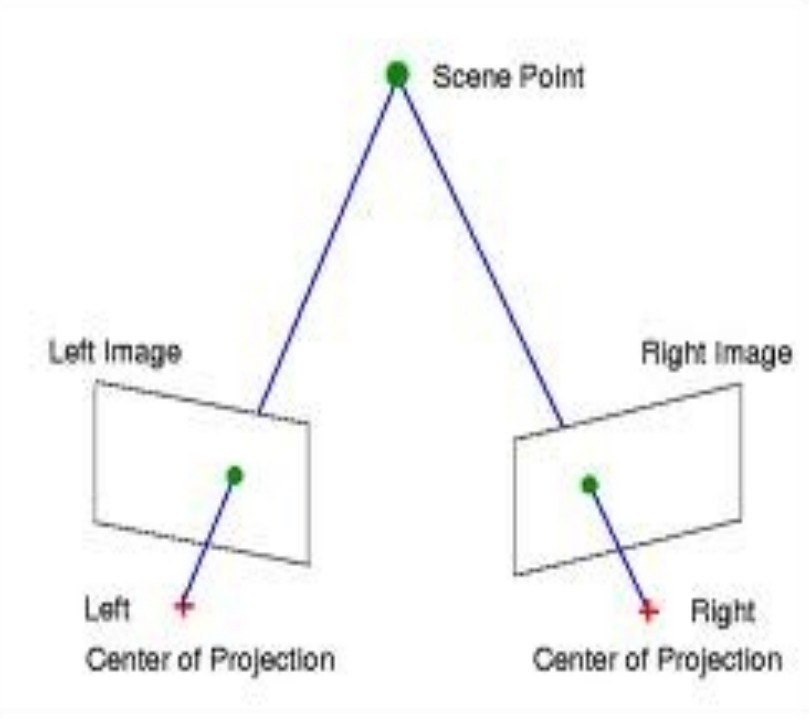
\includegraphics[width=5cm,height=3.3cm]{../Thesis_work/Latex_thesis_work/img_source/stereo_correspondence_abstract.png}}
\hspace{1cm}\subfloat[Stereo-correspondence]{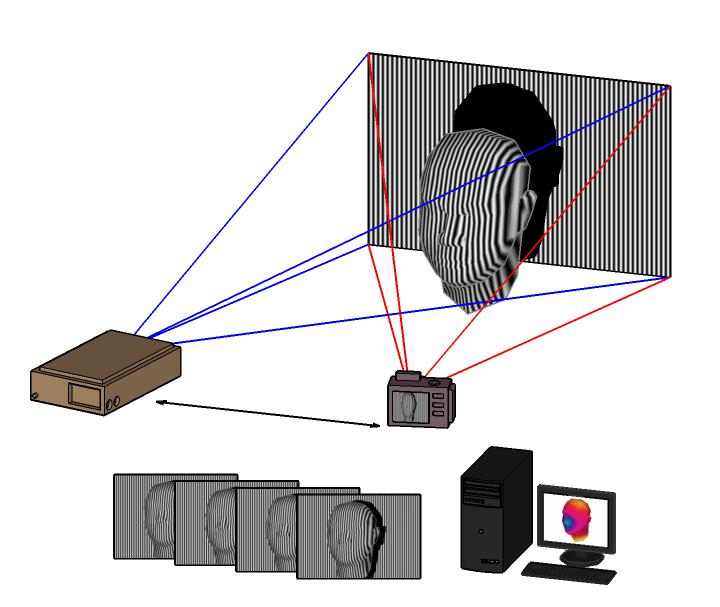
\includegraphics[width=5cm,height=3.3cm]{../Thesis_work/Latex_thesis_work/img_source/phase_shift.jpg}}
\end{figure}
\end{frame}
%%%%%%%%%%%%%%%%%%%%%%%%%%%%%%%%%%%%%%%%%%%%%%%%%%%%%%%%%%%%%%%%%%%%%%%%%%%%SLIDE ENDS%%%%%%%%%%%%%%%%%%%%%%%%%%%%%%%%%%%%%%%

%%%%%%%%%%%%%%%%%%%%%%%%%%%%%%%%%%%%%%%%%%%%%%%%%%%%%%%%%%%%%%%%%%%%%%%%%%%%%SLIDE starts%%%%%%%%%%%%%%%%%%%%%%%%%%%%%%%%%%%%%
\begin{frame}
\frametitle{Architecture of developed system}
\begin{figure}
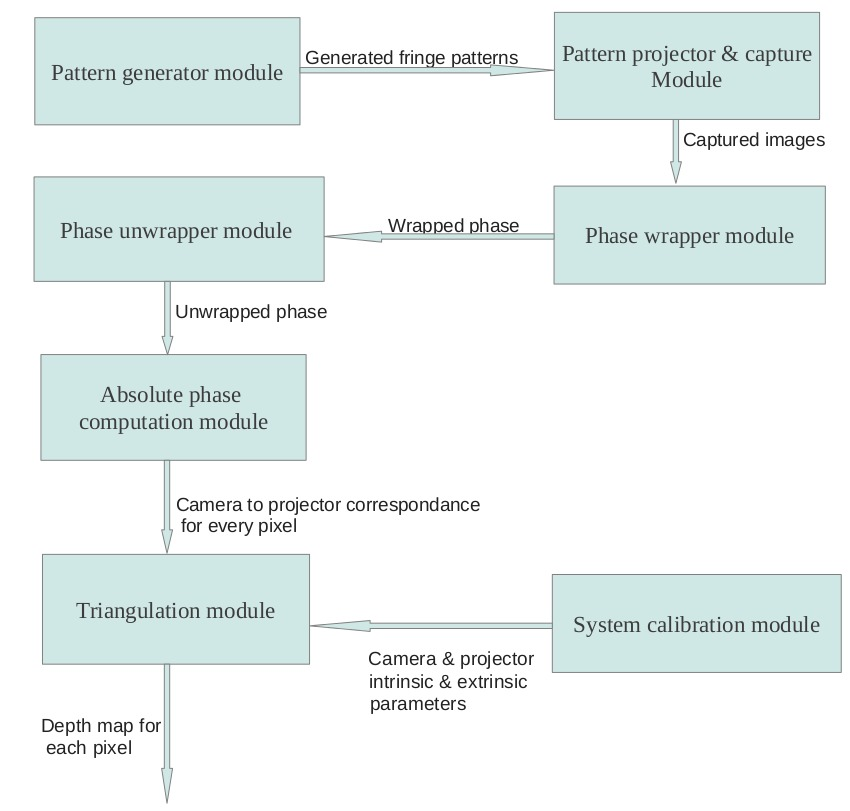
\includegraphics[width=8cm,height=7.5cm]{../Thesis_work/Latex_thesis_work/img_source/system_layout.png}
\caption{System architecture}
\end{figure}
\end{frame}
%%%%%%%%%%%%%%%%%%%%%%%%%%%%%%%%%%%%%%%%%%%%%%%%%%%%%%%%%%%%%%%%%%%%%%%%%%%%SLIDE ENDS%%%%%%%%%%%%%%%%%%%%%%%%%%%%%%%%%%%%%%%

%%%%%%%%%%%%%%%%%%%%%%%%%%%%%%%%%%%%%%%%%%%%%%%%%%%%%%%%%%%%%%%%%%%%%%%%%%%%%SLIDE starts%%%%%%%%%%%%%%%%%%%%%%%%%%%%%%%%%%%%%
\begin{frame}
\frametitle{System setup}
\begin{enumerate}
\item Sharp PG-F200X projector at 1024X768 resolution
\item Logitech Quickcam Sphere AF webcam at 640X480 and 1600X1200 resolutions.
\item Developed system has been used and tested at Core i3-550 processor with 4GB RAM.
\end{enumerate}

\begin{figure}
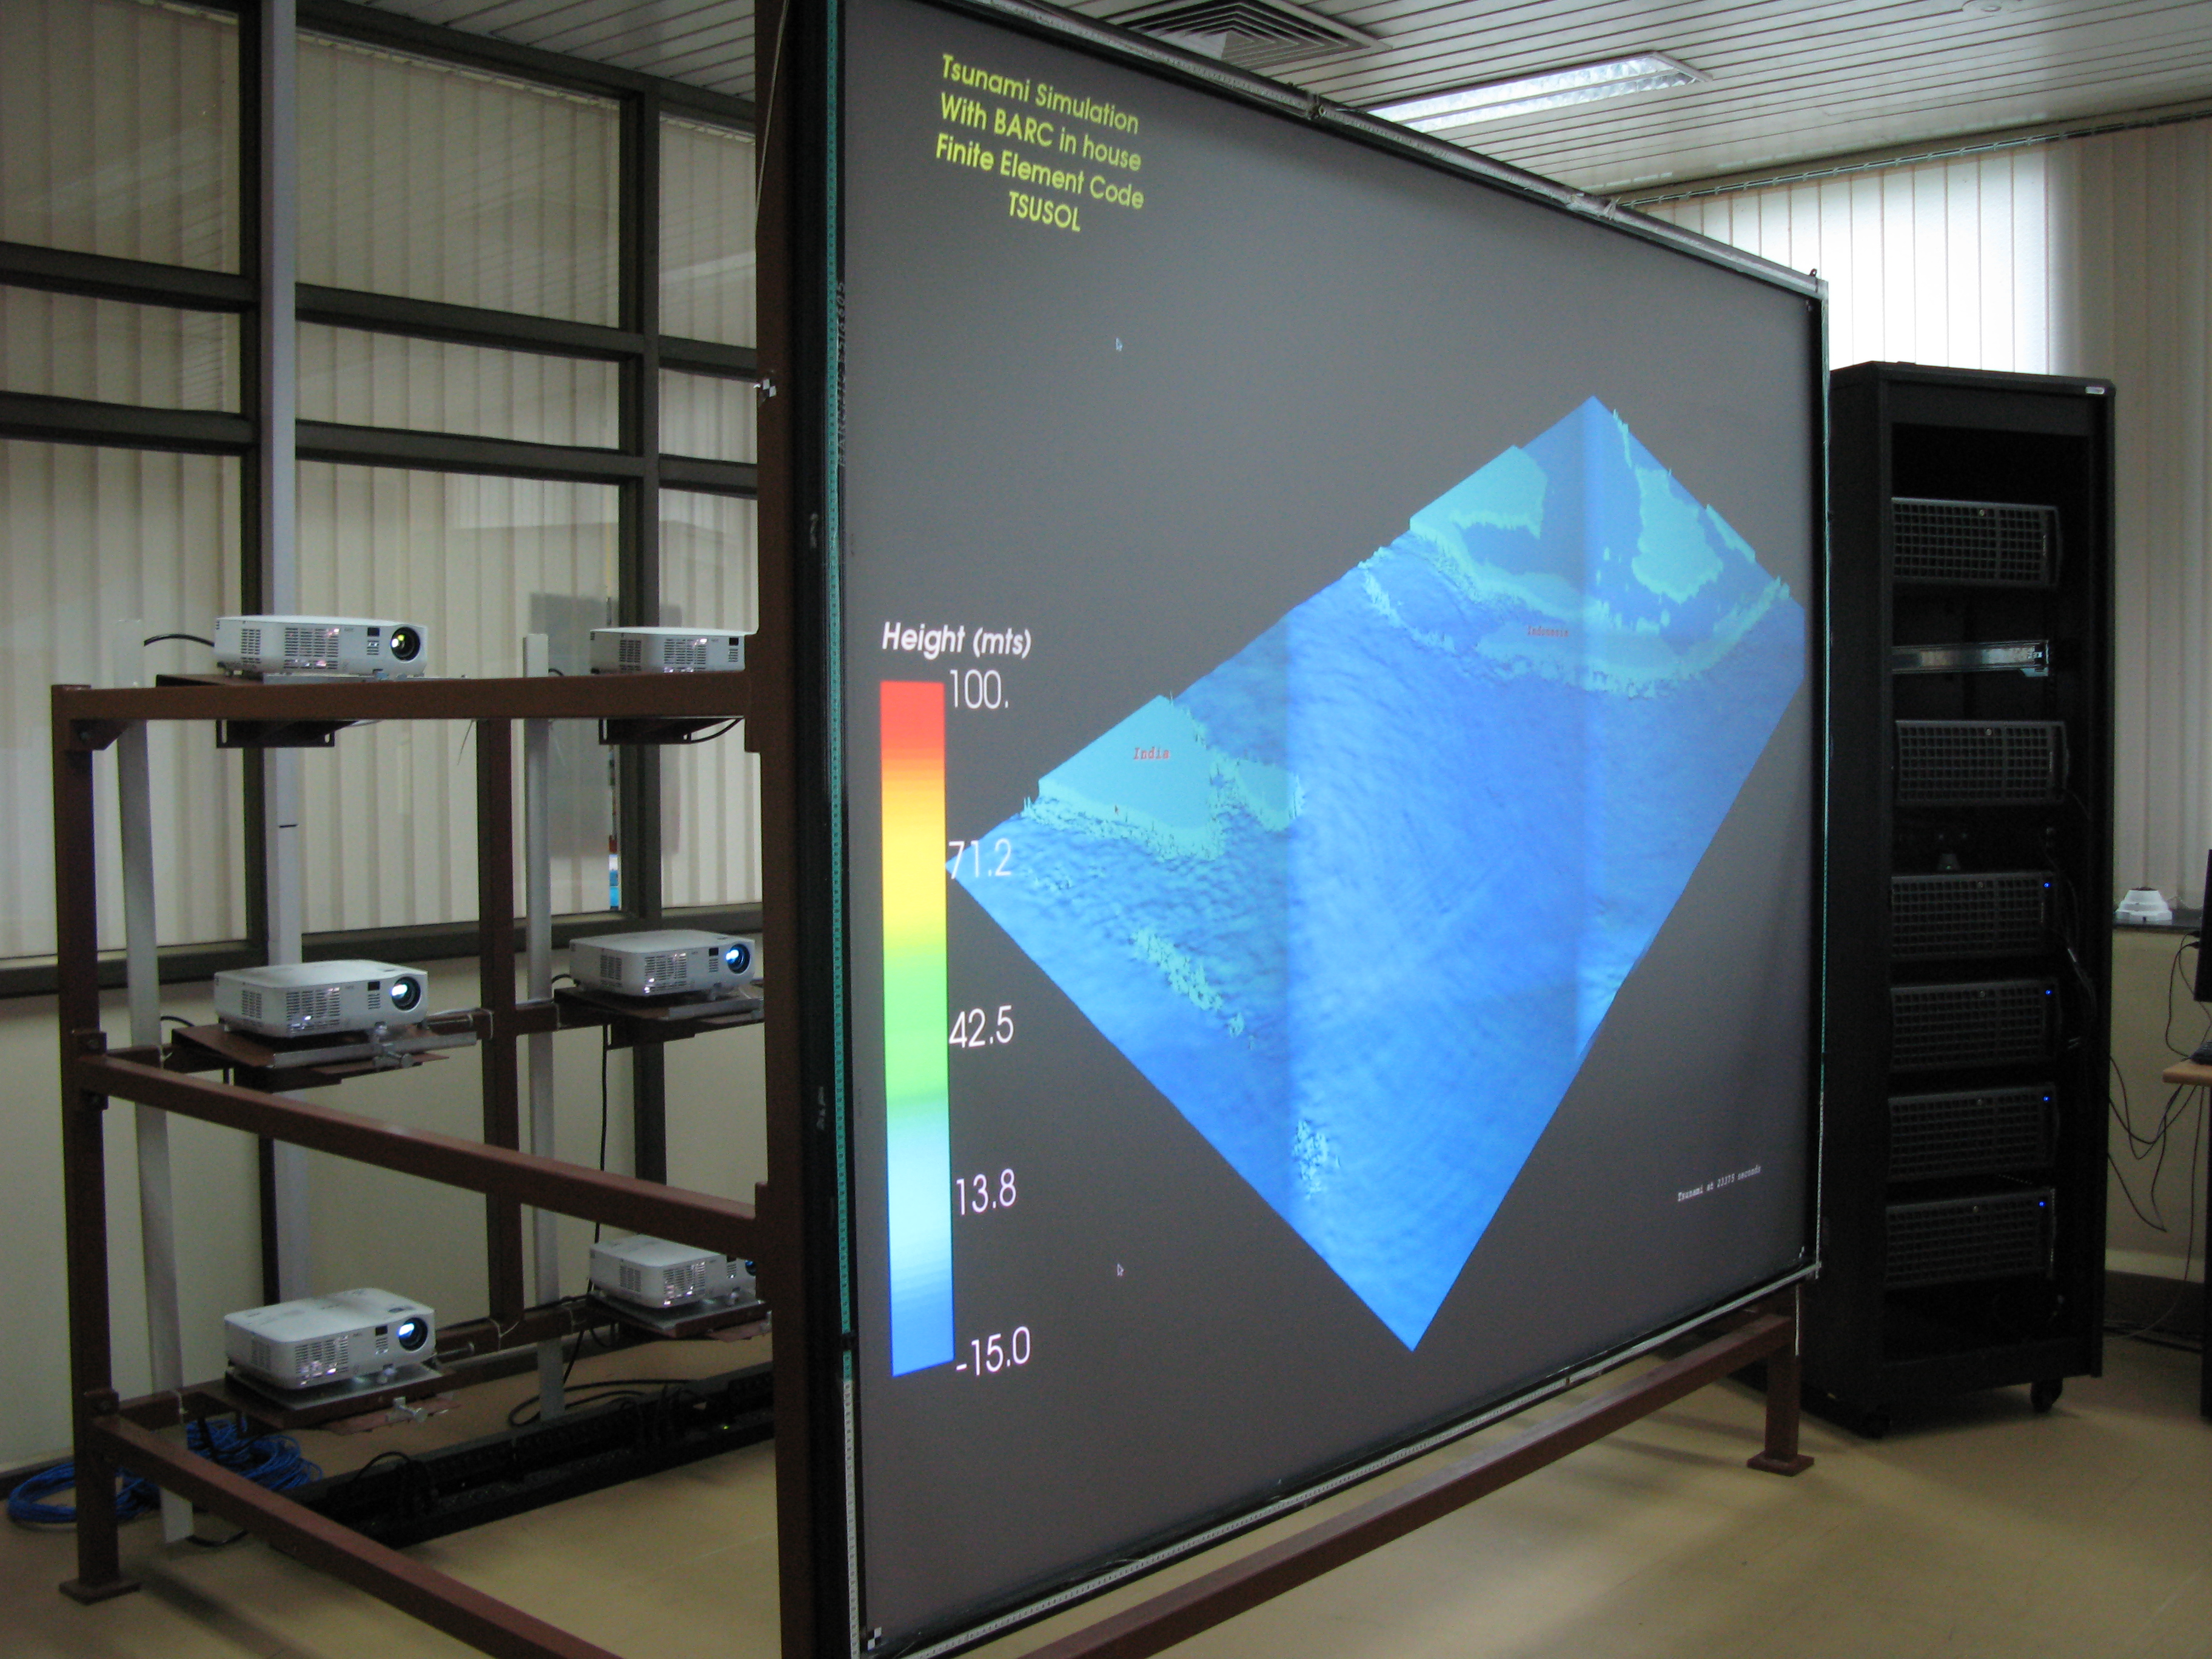
\includegraphics[width=5cm,height=5cm]{../Thesis_work/Latex_thesis_work/img_source/system_setup.png}
\end{figure}
\end{frame}
%%%%%%%%%%%%%%%%%%%%%%%%%%%%%%%%%%%%%%%%%%%%%%%%%%%%%%%%%%%%%%%%%%%%%%%%%%%%SLIDE ENDS%%%%%%%%%%%%%%%%%%%%%%%%%%%%%%%%%%%%%%%


%%%%%%%%%%%%%%%%%%%%%%%%%%%%%%%%%%%%%%%%%%%%%%%%%%%%%%%%%%%%%%%%%%%%%%%%%%%%%SLIDE starts%%%%%%%%%%%%%%%%%%%%%%%%%%%%%%%%%%%%%
\begin{frame}
\frametitle{Pattern generator module}
Vertical phase shifted patterns are defined by:\newline
\begin{equation}
\begin{aligned}
& P_1^v=A_v+B_v*cos(\theta_v-\alpha) \\
& P_2^v=A_v+B_v*cos(\theta_v) \\
& P_3^v=A_v+B_v*cos(\theta_v+\alpha) \\
\end{aligned}
\end{equation}
where $\theta_v=2\pi\frac{x}{fringe\ width}$

\begin{figure}[ht]
%\def\tabularxcolumn#1{m{#1}}
\begin{tabularx}{\linewidth}{@{}cXX@{}}
\begin{tabular}{c c c}
\hspace{1.5cm}\subfloat[]{
\includegraphics[width=3cm,height=3cm]{../Thesis_work/Latex_thesis_work/img_source/phase_ver_1.png}} &
\subfloat[]{
\includegraphics[width=3cm,height=3cm]{../Thesis_work/Latex_thesis_work/img_source/phase_ver_2.png}} &
\subfloat[]{
\includegraphics[width=3cm,height=3cm]{../Thesis_work/Latex_thesis_work/img_source/phase_ver_3.png}} \\ 
\end{tabular}
\end{tabularx}
\caption{Vertical phase-shifted patterns}
\label{fig:vert_phase_pattern}
\end{figure}
\end{frame}
%%%%%%%%%%%%%%%%%%%%%%%%%%%%%%%%%%%%%%%%%%%%%%%%%%%%%%%%%%%%%%%%%%%%%%%%%%%%SLIDE ENDS%%%%%%%%%%%%%%%%%%%%%%%%%%%%%%%%%%%%%%%


%%%%%%%%%%%%%%%%%%%%%%%%%%%%%%%%%%%%%%%%%%%%%%%%%%%%%%%%%%%%%%%%%%%%%%%%%%%%%SLIDE starts%%%%%%%%%%%%%%%%%%%%%%%%%%%%%%%%%%%%%
\begin{frame}
Horizontal phase-shifted patterns are defined by:\newline
\begin{equation}
\begin{aligned}
& P_1^h=A_h+B_h*cos(\theta_h-\alpha) \\
& P_2^h=A_h+B_h*cos(\theta_h) \\
& P_3^h=A_h+B_h*cos(\theta_h+\alpha) \\
\end{aligned}
\end{equation}
where $\theta_h=2\pi\frac{y}{fringe\ width}$

\begin{figure}[ht]
%\def\tabularxcolumn#1{m{#1}}
\begin{tabularx}{\linewidth}{@{}cXX@{}}
\begin{tabular}{c c c}
\hspace{1.5cm}\subfloat[]{
\includegraphics[width=3cm,height=3cm]{../Thesis_work/Latex_thesis_work/img_source/phase_hor_1.png}} &
\subfloat[]{
\includegraphics[width=3cm,height=3cm]{../Thesis_work/Latex_thesis_work/img_source/phase_hor_2.png}} &
\subfloat[]{
\includegraphics[width=3cm,height=3cm]{../Thesis_work/Latex_thesis_work/img_source/phase_hor_3.png}} \\ 
\end{tabular}
\end{tabularx}
\caption{Horizontal phase-shifted patterns}
\label{fig:horz_phase_pattern}
\end{figure}
\end{frame}
%%%%%%%%%%%%%%%%%%%%%%%%%%%%%%%%%%%%%%%%%%%%%%%%%%%%%%%%%%%%%%%%%%%%%%%%%%%%SLIDE ENDS%%%%%%%%%%%%%%%%%%%%%%%%%%%%%%%%%%%%%%%



%%%%%%%%%%%%%%%%%%%%%%%%%%%%%%%%%%%%%%%%%%%%%%%%%%%%%%%%%%%%%%%%%%%%%%%%%%%%SLIDE starts%%%%%%%%%%%%%%%%%%%%%%%%%%%%%%%%%%%%%%%
\begin{frame}
Vertical binary coded patterns are defined by:\newline
\begin{equation}
N_{v}^{codes}=\frac{W_{projector}}{w_{fringe}} 
\end{equation}
\begin{equation}
N_{v}^{patterns}=\log_2(N_v^{codes})
\end{equation}
\begin{equation}
Intensity_{(i,j)}=\lfloor i/{(w_{fringe}*2^{pattern\ number})} \rfloor
\end{equation}
\begin{figure}[ht]
\begin{tabularx}{\linewidth}{@{}cXX@{}}
\begin{tabular}{c c c}
\hspace{1.5cm}\subfloat[]{
\includegraphics[width=3cm,height=3cm]{../Thesis_work/Latex_thesis_work/img_source/binary_ver_1.png}} &
\subfloat[]{
\includegraphics[width=3cm,height=3cm]{../Thesis_work/Latex_thesis_work/img_source/binary_ver_2.png}} &
\subfloat[]{
\includegraphics[width=3cm,height=3cm]{../Thesis_work/Latex_thesis_work/img_source/binary_ver_3.png}} \\
\end{tabular}
\end{tabularx}
\caption{Vertical phase shifted patterns}
\end{figure}

\end{frame}
%%%%%%%%%%%%%%%%%%%%%%%%%%%%%%%%%%%%%%%%%%%%%%%%%%%%%%%%%%%%%%%%%%%%%%%%%%%%SLIDE ENDS%%%%%%%%%%%%%%%%%%%%%%%%%%%%%%%%%%%%%%%



%%%%%%%%%%%%%%%%%%%%%%%%%%%%%%%%%%%%%%%%%%%%%%%%%%%%%%%%%%%%%%%%%%%%%%%%%%%%%SLIDE starts%%%%%%%%%%%%%%%%%%%%%%%%%%%%%%%%%%%%%
\begin{frame}
Horizontal binary coded patterns are defined by:\newline
\begin{equation}
N_h^{codes}=\frac{H_{projector}}{w_{fringe}} 
\end{equation}
\begin{equation}
N_{h}^{patterns}=\log_2(N_h^{codes})
\end{equation}

\begin{equation}
Intensity_{(i,j)}=\lfloor j/{(w_{fringe}*2^{pattern\ number})} \rfloor
\end{equation}

\begin{figure}[ht]
\begin{tabularx}{\linewidth}{@{}cXX@{}}
\begin{tabular}{c c c}
\hspace{1.5cm}\subfloat[]{
\includegraphics[width=3cm,height=3cm]{../Thesis_work/Latex_thesis_work/img_source/binary_hor_1.png}} &
\subfloat[]{
\includegraphics[width=3cm,height=3cm]{../Thesis_work/Latex_thesis_work/img_source/binary_hor_2.png}} &
\subfloat[]{
\includegraphics[width=3cm,height=3cm]{../Thesis_work/Latex_thesis_work/img_source/binary_hor_3.png}} \\
\end{tabular}
\end{tabularx}
\caption{Horizontal binary coded patterns}
\end{figure}
\end{frame}
%%%%%%%%%%%%%%%%%%%%%%%%%%%%%%%%%%%%%%%%%%%%%%%%%%%%%%%%%%%%%%%%%%%%%%%%%%%%SLIDE ENDS%%%%%%%%%%%%%%%%%%%%%%%%%%%%%%%%%%%%%%%

%%%%%%%%%%%%%%%%%%%%%%%%%%%%%%%%%%%%%%%%%%%%%%%%%%%%%%%%%%%%%%%%%%%%%%%%%%%%%SLIDE starts%%%%%%%%%%%%%%%%%%%%%%%%%%%%%%%%%%%%%
\begin{frame}
\frametitle{Pattern projection and capture module}
\begin{figure}
\begin{tabularx}{\linewidth}{@{}cXX@{}}
\begin{tabular}{c c c}
\hspace{1cm}\subfloat[]{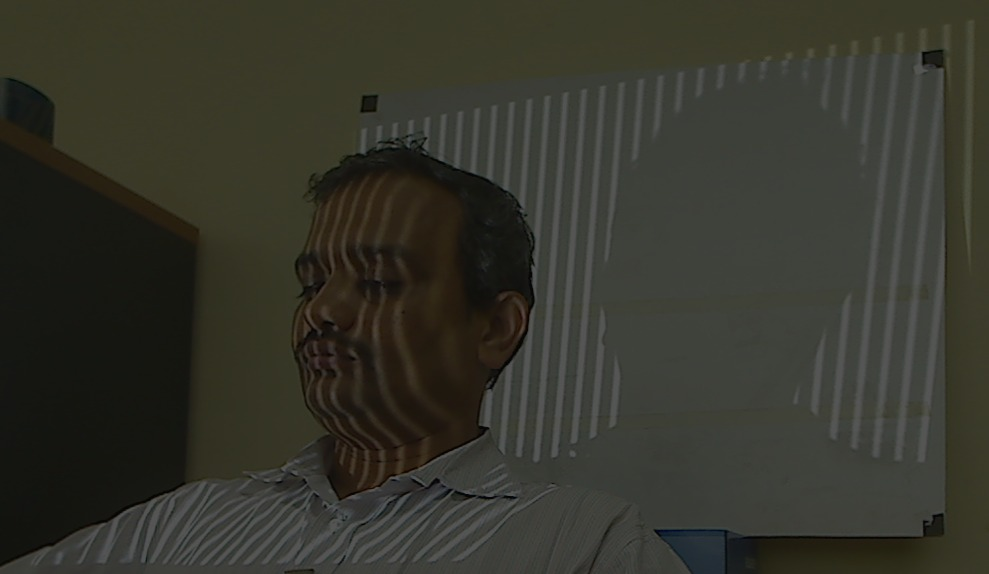
\includegraphics[width=3cm,height=3cm]{../Thesis_work/Latex_thesis_work/img_source/cap_fringe_1.png}} &
\subfloat[]{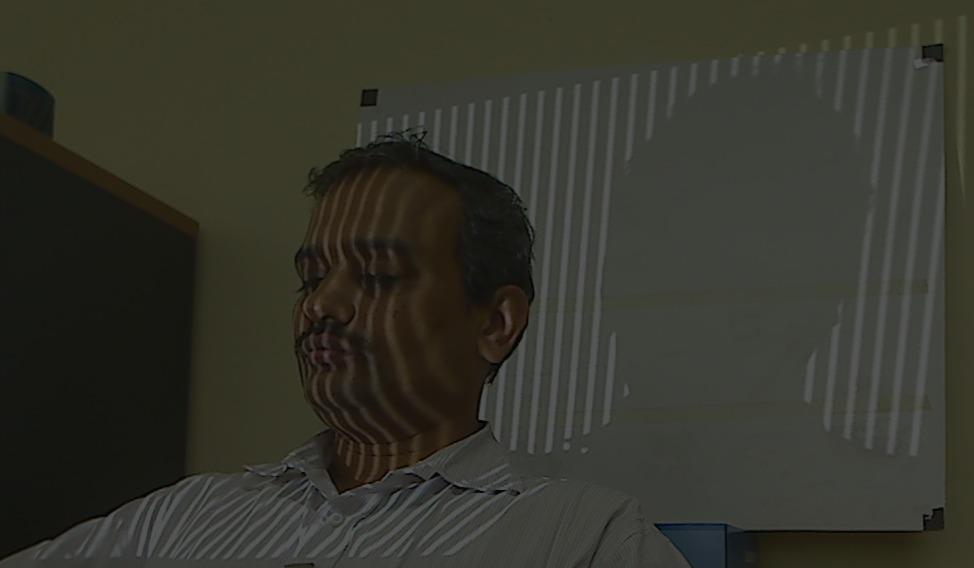
\includegraphics[width=3cm,height=3cm]{../Thesis_work/Latex_thesis_work/img_source/cap_fringe_2.png}} &
\subfloat[]{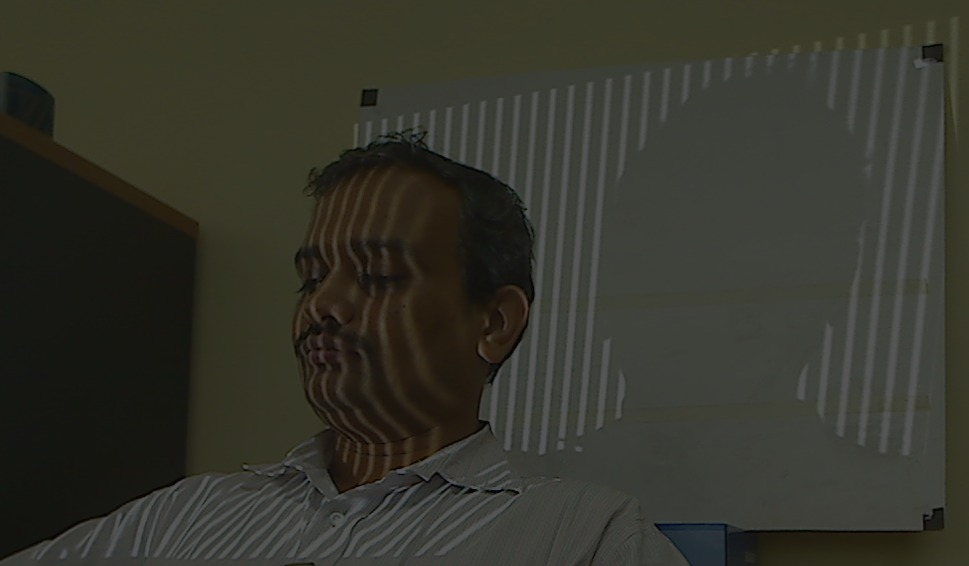
\includegraphics[width=3cm,height=3cm]{../Thesis_work/Latex_thesis_work/img_source/cap_fringe_3.png}} \\
\hspace{1cm}\subfloat[]{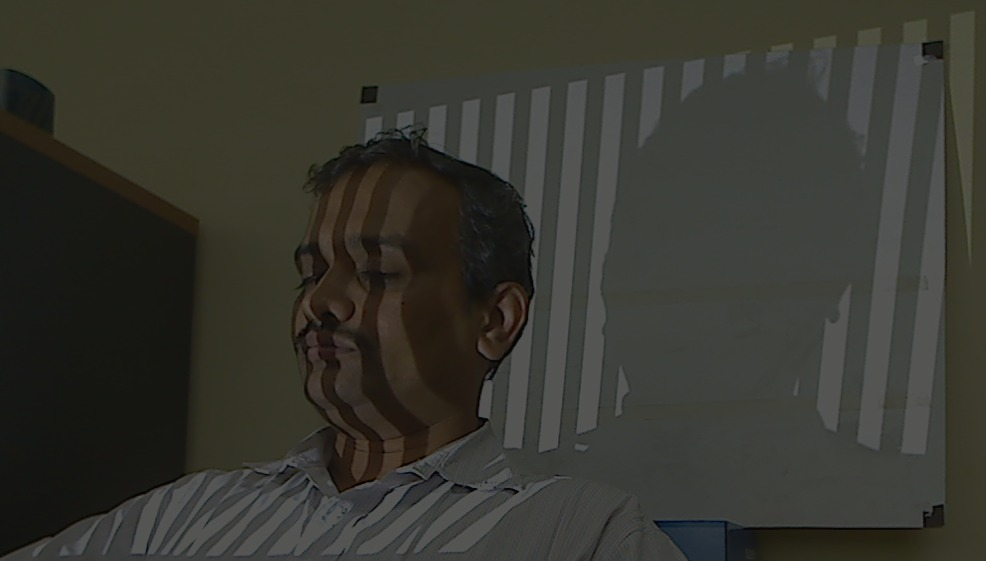
\includegraphics[width=3cm,height=3cm]{../Thesis_work/Latex_thesis_work/img_source/cap_fringe_4.png}} &
\subfloat[]{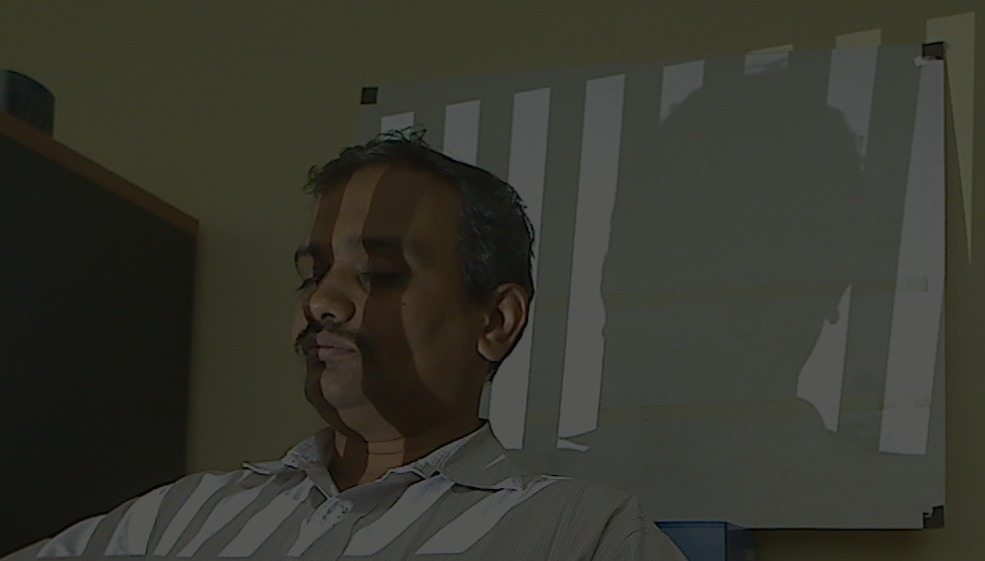
\includegraphics[width=3cm,height=3cm]{../Thesis_work/Latex_thesis_work/img_source/cap_fringe_5.png}} &
\subfloat[]{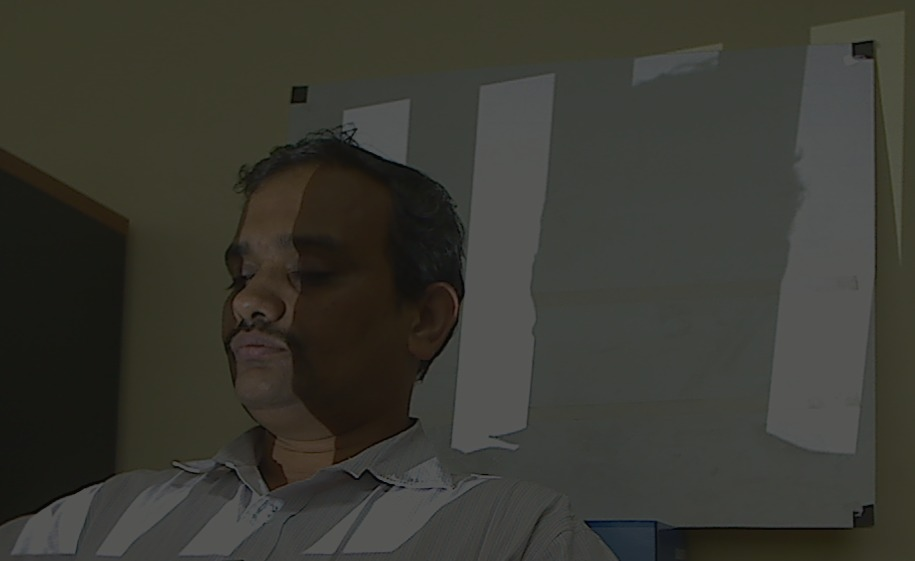
\includegraphics[width=3cm,height=3cm]{../Thesis_work/Latex_thesis_work/img_source/cap_fringe_6.png}} \\
\end{tabular}
\end{tabularx}
\caption{Captured vertical phase-shifted and binary coded patterns}
\end{figure}
\end{frame}
%%%%%%%%%%%%%%%%%%%%%%%%%%%%%%%%%%%%%%%%%%%%%%%%%%%%%%%%%%%%%%%%%%%%%%%%%%%%SLIDE ENDS%%%%%%%%%%%%%%%%%%%%%%%%%%%%%%%%%%%%%%%

%%%%%%%%%%%%%%%%%%%%%%%%%%%%%%%%%%%%%%%%%%%%%%%%%%%%%%%%%%%%%%%%%%%%%%%%%%%%%SLIDE starts%%%%%%%%%%%%%%%%%%%%%%%%%%%%%%%%%%%%%
\begin{frame}
\begin{figure}
\begin{tabularx}{\linewidth}{@{}cXX@{}}
\begin{tabular}{c c c}
\hspace{1cm}\subfloat[]{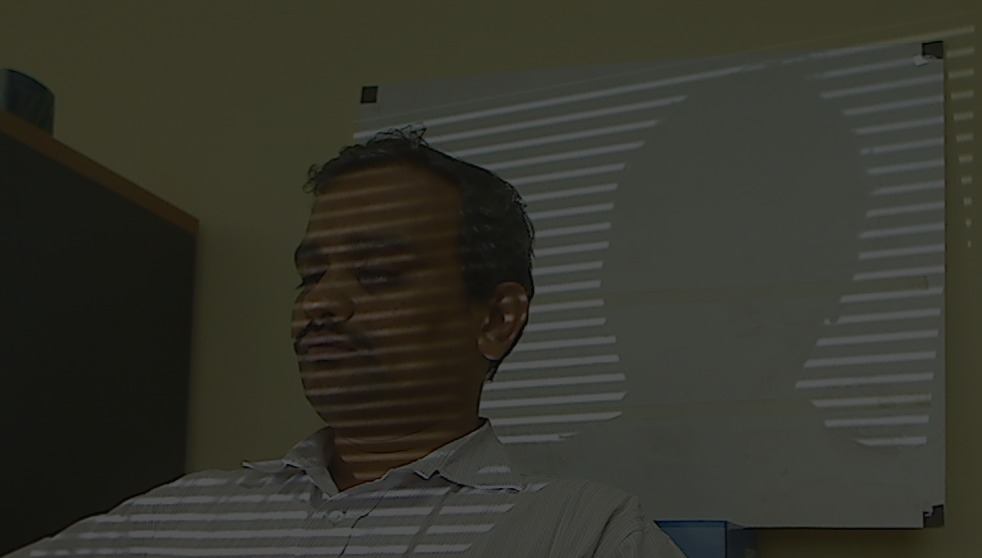
\includegraphics[width=3cm,height=3cm]{../Thesis_work/Latex_thesis_work/img_source/cap_binary_1.png}} &
\subfloat[]{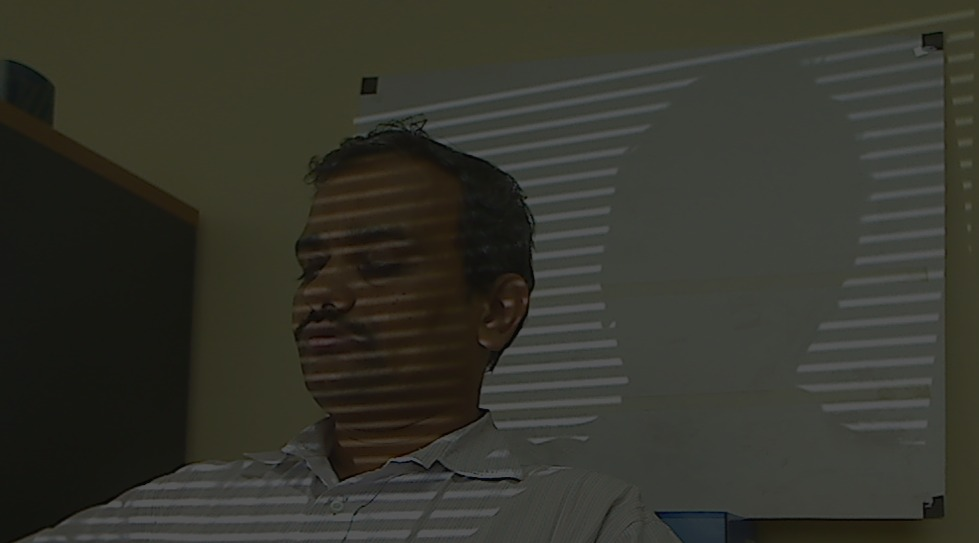
\includegraphics[width=3cm,height=3cm]{../Thesis_work/Latex_thesis_work/img_source/cap_binary_2.png}} &
\subfloat[]{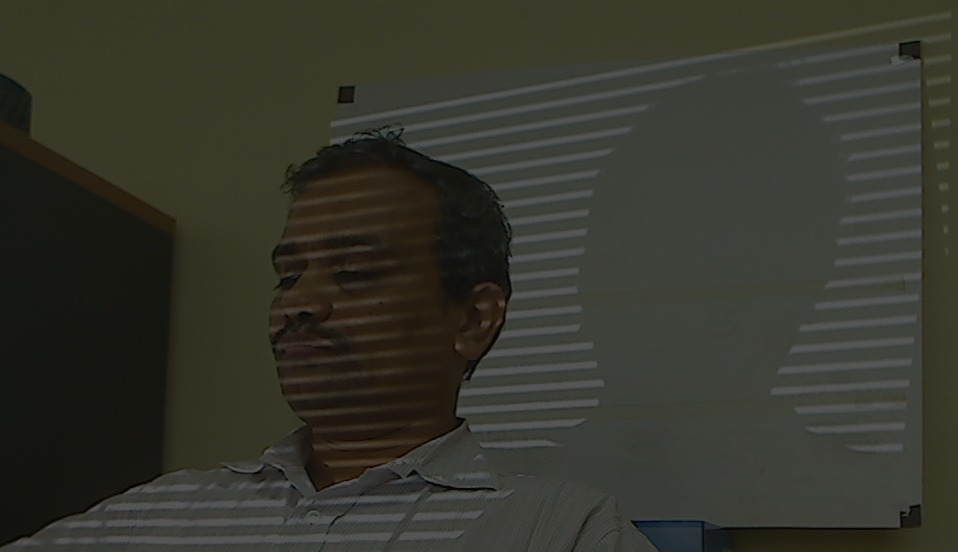
\includegraphics[width=3cm,height=3cm]{../Thesis_work/Latex_thesis_work/img_source/cap_binary_3.png}} \\
\hspace{1cm}\subfloat[]{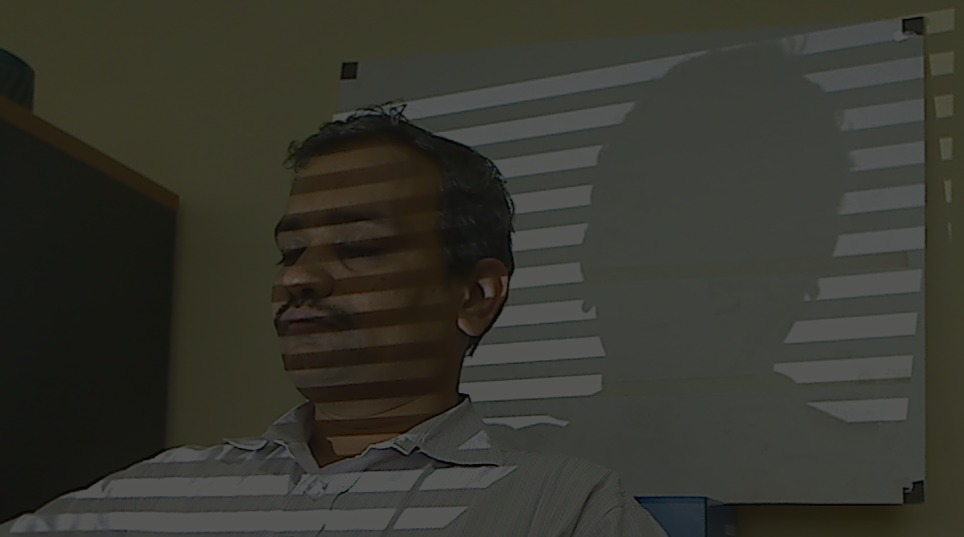
\includegraphics[width=3cm,height=3cm]{../Thesis_work/Latex_thesis_work/img_source/cap_binary_4.png}} &
\subfloat[]{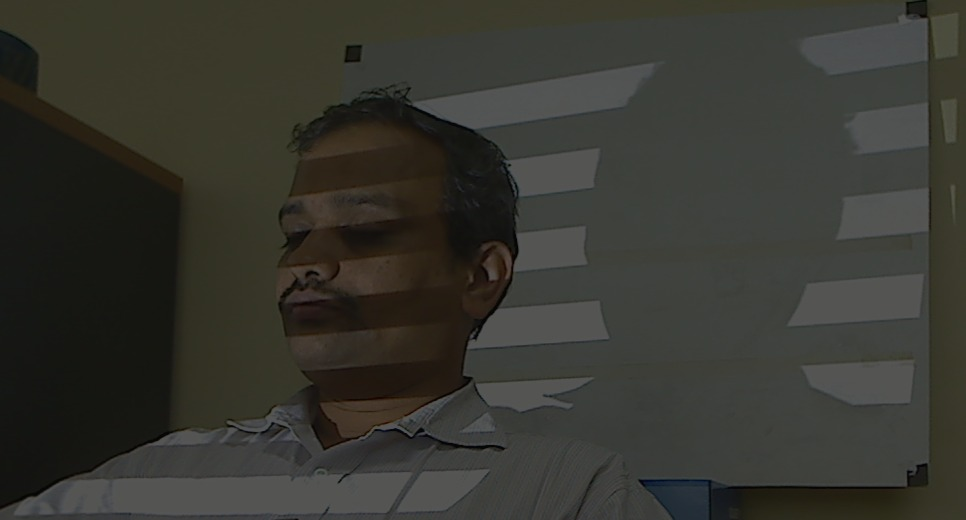
\includegraphics[width=3cm,height=3cm]{../Thesis_work/Latex_thesis_work/img_source/cap_binary_5.png}} &
\subfloat[]{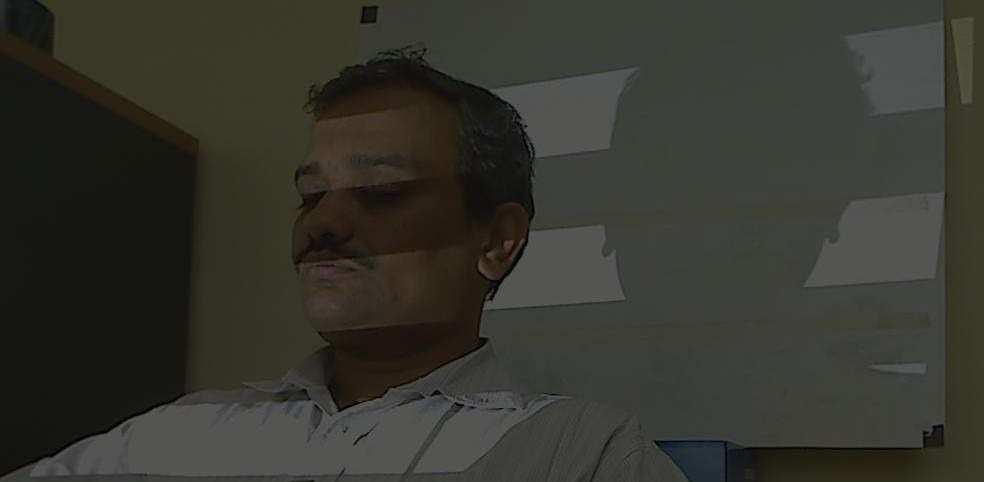
\includegraphics[width=3cm,height=3cm]{../Thesis_work/Latex_thesis_work/img_source/cap_binary_6.png}}
\end{tabular}
\end{tabularx}
\caption{Captured horizontal phase-shifted and binary coded patterns}
\end{figure}
\end{frame}
%%%%%%%%%%%%%%%%%%%%%%%%%%%%%%%%%%%%%%%%%%%%%%%%%%%%%%%%%%%%%%%%%%%%%%%%%%%%SLIDE ENDS%%%%%%%%%%%%%%%%%%%%%%%%%%%%%%%%%%%%%%%


%%%%%%%%%%%%%%%%%%%%%%%%%%%%%%%%%%%%%%%%%%%%%%%%%%%%%%%%%%%%%%%%%%%%%%%%%%%%%SLIDE starts%%%%%%%%%%%%%%%%%%%%%%%%%%%%%%%%%%%%%
\begin{frame}
\frametitle{Phase wrapping module}
Assumed illumination model for 3 phase shifted pattern approach:
\begin{equation}
\begin{aligned}
& I_1^{v/h}=I_{dc}^{v/h}+I_{mod}^{v/h}*cos(\theta_{v/h}-\alpha) \\
& I_2^{v/h}=I_{dc}^{v/h}+I_{mod}^{v/h}*cos(\theta_{v/h}) \\
& I_3^{v/h}=I_{dc}^{v/h}+I_{mod}^{v/h}*cos(\theta_{v/h}+\alpha)
\end{aligned}
\end{equation}
Hence,
\begin{equation}
\begin{aligned}
& \theta_v=tan^{-1}\bigg[\frac{\sqrt[2]{3}(I_1^v-I_3^v)}{2I_2^v-I_1^v-I_3^v}\bigg],-\pi\leq\theta_v\leq\pi,
& \theta_h=tan^{-1}\bigg[\frac{\sqrt[2]{3}(I_1^h-I_3^h)}{2I_2^h-I_1^h-I_3^h}\bigg],-\pi\leq\theta_h\leq\pi 
\end{aligned}
\end{equation}
\begin{figure}[ht]
%\def\tabularxcolumn#1{m{#1}}
\begin{tabularx}{\linewidth}{@{}cXX@{}}
\begin{tabular}{l r}
\hspace{3cm}\subfloat[Vertical wrapped phase]{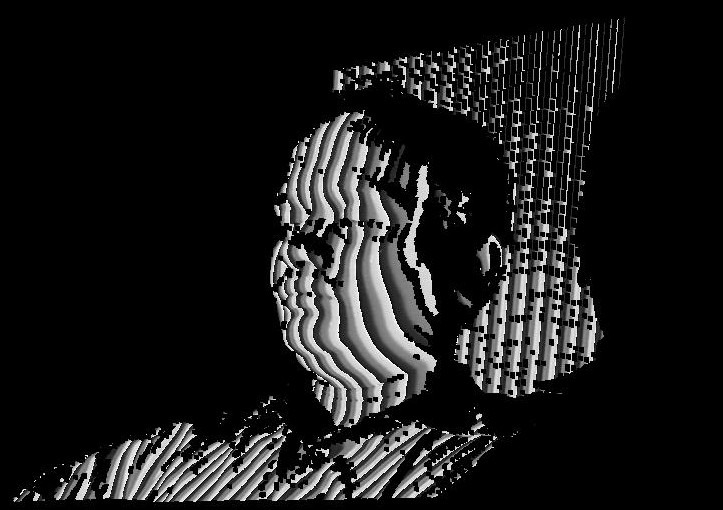
\includegraphics[width=3cm,height=3cm]{../Thesis_work/Latex_thesis_work/img_source/wrapped_ver.png}} &
\subfloat[Horizontal wrapped phase]{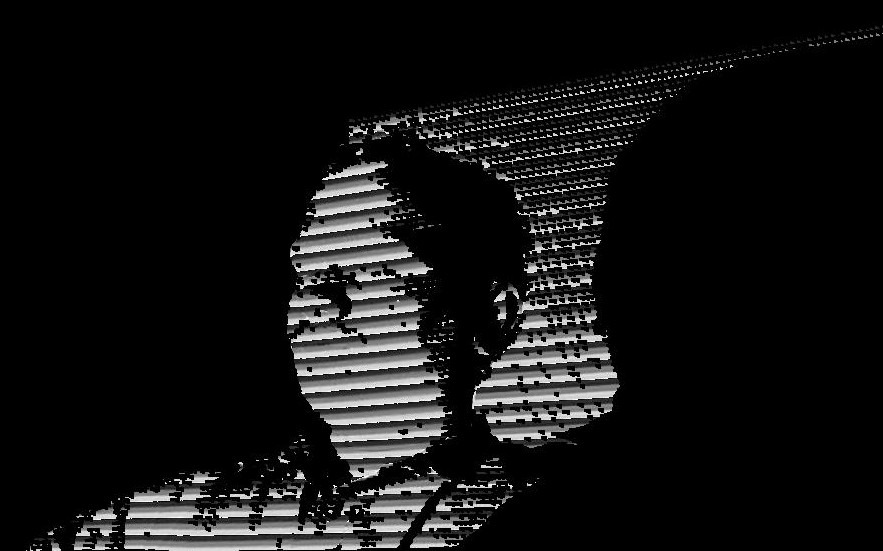
\includegraphics[width=3cm,height=3cm]{../Thesis_work/Latex_thesis_work/img_source/wrapped_hor.png}}\\
\end{tabular}
\end{tabularx}
\caption{Computed wrapped phase}
\label{fig:wrapped_phase}
\end{figure}
\end{frame}
%%%%%%%%%%%%%%%%%%%%%%%%%%%%%%%%%%%%%%%%%%%%%%%%%%%%%%%%%%%%%%%%%%%%%%%%%%%%SLIDE ENDS%%%%%%%%%%%%%%%%%%%%%%%%%%%%%%%%%%%%%%%

%%%%%%%%%%%%%%%%%%%%%%%%%%%%%%%%%%%%%%%%%%%%%%%%%%%%%%%%%%%%%%%%%%%%%%%%%%%%%SLIDE starts%%%%%%%%%%%%%%%%%%%%%%%%%%%%%%%%%%%%%
\begin{frame}
\frametitle{Phase unwrapping module}
Unwrapped phase $(\psi_v,\psi_h)$ maps $(\theta_v,\theta_h)$ to its correct $2\pi$ multiple:
\begin{equation}
\begin{aligned}
& \psi_v=\theta_v+2\pi*C_v \\
& \psi_h=\theta_h+2\pi*C_h
\end{aligned}
\end{equation}
where,\newline
\indent 
$C_v(x,y)$: Decoded vertical binary code(or \textit{vertical period number}) at any pixel (x,y).\newline
$C_h(x,y)$: Decoded horizontal binary code(or \textit{horizontal period number}) at any pixel (x,y).
\begin{figure}[ht]
%\def\tabularxcolumn#1{m{#1}}
\begin{tabularx}{\linewidth}{@{}cXX@{}}
\begin{tabular}{l r}
\hspace{3cm}\subfloat[Vertical unwrapped phase]{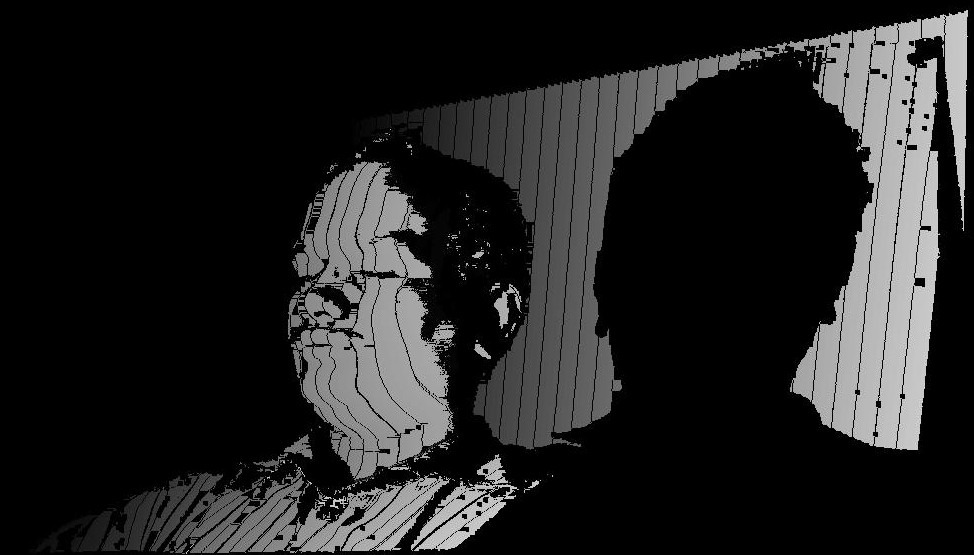
\includegraphics[width=3cm,height=3cm]{../Thesis_work/Latex_thesis_work/img_source/unwrapped_ver.png}} &
\subfloat[Horizontal unwrapped phase]{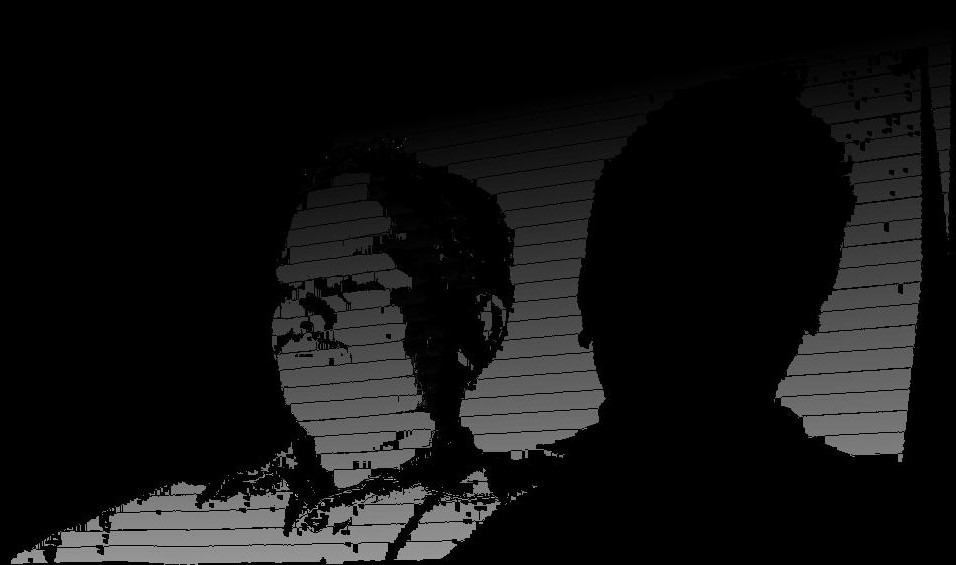
\includegraphics[width=3cm,height=3cm]{../Thesis_work/Latex_thesis_work/img_source/unwrapped_hor.png}}\\
\end{tabular}
\end{tabularx}
\caption{Computed unwrapped phase}
\label{fig:unwrapped_phase}
\end{figure}
\end{frame}
%%%%%%%%%%%%%%%%%%%%%%%%%%%%%%%%%%%%%%%%%%%%%%%%%%%%%%%%%%%%%%%%%%%%%%%%%%%%SLIDE ENDS%%%%%%%%%%%%%%%%%%%%%%%%%%%%%%%%%%%%%%%

%%%%%%%%%%%%%%%%%%%%%%%%%%%%%%%%%%%%%%%%%%%%%%%%%%%%%%%%%%%%%%%%%%%%%%%%%%%%%SLIDE starts%%%%%%%%%%%%%%%%%%%%%%%%%%%%%%%%%%%%%
\begin{frame}
\frametitle{Absolute phase computation module}
Computing projector coordinates $(X_p,Y_p)$ corresponding to a camera coordinates $(X_c,Y_c)$
\begin{equation}
\begin{aligned}
& X_p=\lfloor w_{fringe}*\big(\frac{\psi_v}{2\pi}\big) \rfloor  ,
%2\pi*\bigg\lfloor\frac{\psi_v(X_c,Y_c)}{2\pi}\bigg\rfloor+2\pi*\bigg(\frac{\psi_v(X_c,Y_c)}{2\pi}-\bigg\lfloor\frac{\psi_v(X_c,Y_c)}{2\pi}\bigg\rfloor\bigg) \\
& Y_p=\lfloor w_{fringe}*\big(\frac{\psi_h}{2\pi}\big) \rfloor%2\pi*\bigg\lfloor\frac{\psi_h(X_c,Y_c)}{2\pi}\bigg\rfloor+2\pi*\bigg(\frac{\psi_h(X_c,Y_c)}{2\pi}-\bigg\lfloor\frac{\psi_h(X_c,Y_c)}{2\pi}\bigg\rfloor\bigg)
\end{aligned}
\end{equation}
\begin{figure}
%\def\tabularxcolumn#1{m{#1}}
\begin{tabularx}{\linewidth}{@{}cXX@{}}
\begin{tabular}{c c}
\hspace{2cm}
\subfloat[Camera image]{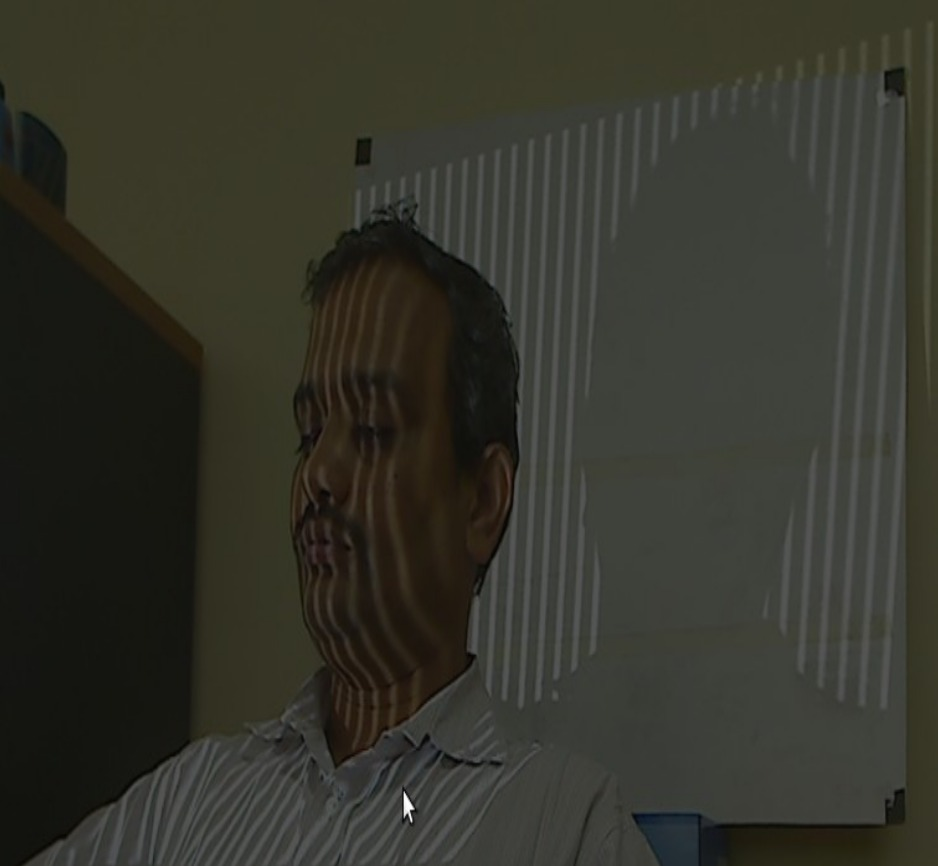
\includegraphics[width=3cm,height=3cm]{../Thesis_work/Latex_thesis_work/img_source/camera_image.png}} &
\subfloat[Projector image]{
\includegraphics[width=3cm,height=3cm]{../Thesis_work/Latex_thesis_work/img_source/projector_image.png}} 
\end{tabular}
\end{tabularx}
\caption{Stereo correspondence between camera and projector}
\label{fig:estimated_correspondence}
\end{figure}
\end{frame}
%%%%%%%%%%%%%%%%%%%%%%%%%%%%%%%%%%%%%%%%%%%%%%%%%%%%%%%%%%%%%%%%%%%%%%%%%%%%SLIDE ENDS%%%%%%%%%%%%%%%%%%%%%%%%%%%%%%%%%%%%%%%


%%%%%%%%%%%%%%%%%%%%%%%%%%%%%%%%%%%%%%%%%%%%%%%%%%%%%%%%%%%%%%%%%%%%%%%%%%%%%SLIDE starts%%%%%%%%%%%%%%%%%%%%%%%%%%%%%%%%%%%%%
\begin{frame}
\frametitle{System calibration module}
\textbf{Intrinsic parameters}\newline  
$f_x$: focal length of lens expressed in number of pixels along X - axis\newline  
$f_y$: focal length of lens expressed in number of pixels along Y - axis\newline  
$(c_x , c_y)$: Pixel coordinates of principal point\newline  
$(k_1, k_2, k_3)$: Radial distortion coefficients\newline  
$(p_1,p_2)$: Tangential distortion coefficients\newline  
\textbf{Extrinsic parameters}\newline  
$(r_x,r_y,r_z)$: Rotation vector between camera(or projector) \& world coordinate system\newline  
$(t_x,t_y,t_z)$: Translation vector between camera(or projector) \& world coordinate system 
\begin{figure}
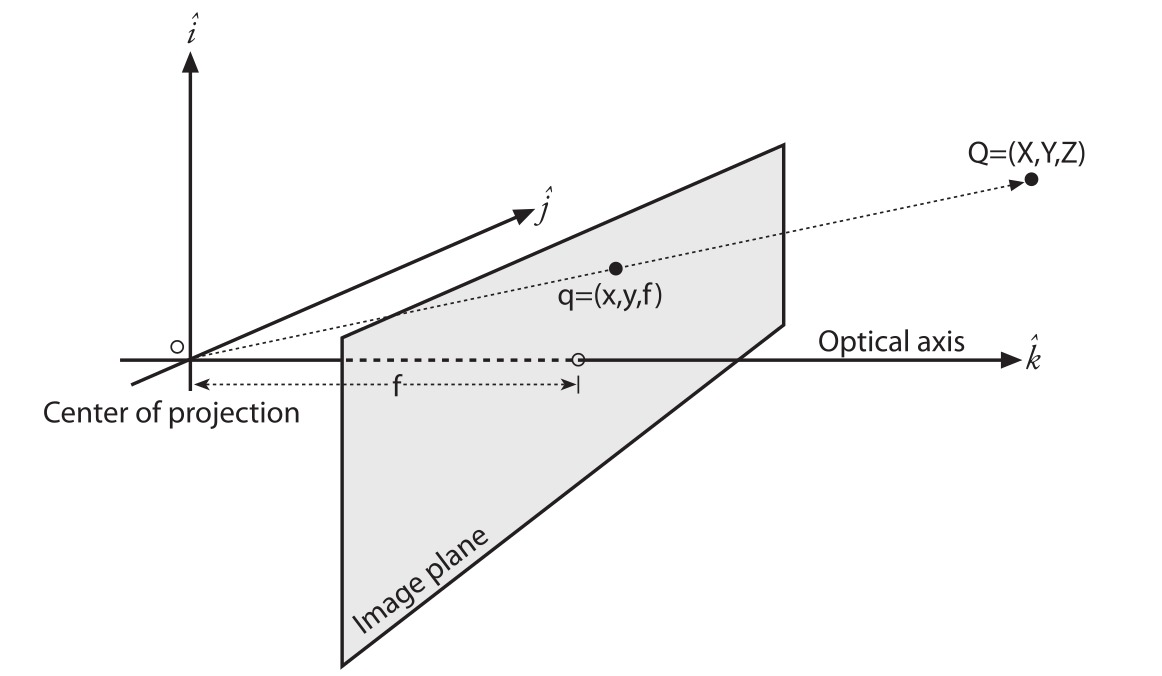
\includegraphics[width=7cm,height=4cm]{../Thesis_work/Latex_thesis_work/img_source/camera_model.png}
\caption{Pin-hole camera model}
\end{figure}
\end{frame}
%%%%%%%%%%%%%%%%%%%%%%%%%%%%%%%%%%%%%%%%%%%%%%%%%%%%%%%%%%%%%%%%%%%%%%%%%%%%SLIDE ENDS%%%%%%%%%%%%%%%%%%%%%%%%%%%%%%%%%%%%%%%
%%%%%%%%%%%%%%%%%%%%%%%%%%%%%%%%%%%%%%%%%%%%%%%%%%%%%%%%%%%%%%%%%%%%%%%%%%%%%SLIDE starts%%%%%%%%%%%%%%%%%%%%%%%%%%%%%%%%%%%%%
\begin{frame}
Mathematically,camera(or projector) model:
\begin{equation}
\begin{aligned}
& \begin{bmatrix}
U_e^i \\
V_e^i
\end{bmatrix} 
=A_c[R|T]\begin{bmatrix}
X_w^i \\
Y_w^i \\
Z_w^i
\end{bmatrix} \\
& \begin{bmatrix}
X_e^i \\
Y_e^i
\end{bmatrix}
=f(U_e^i,V_e^i)
\end{aligned}
\end{equation}

%Abstract description of intrinsic parameter calibration algorithm(OpenCV):
%\begin{enumerate}
%\item Computes the initial intrinsic parameters(assuming zero distortion coefficients).
%\item The initial camera pose is estimated as if the intrinsic parameters have been already known.
%\item Then the global \textit{Levenberg-Marquardt optimization algorithm} is run to minimize the \textit{reprojection error}.
%\end{enumerate}
OpenCV camera calibration algorithm is used which minimizes:\newline
\begin{equation}
\varepsilon=\sum_{i=1}^{N}\bigg[\sqrt[2]{(observed_x-projected_x)^2+(observed_y-projected_y)^2}\bigg]
\end{equation}
Extrinsic parameters that minimize reprojection error are considered as the \textit{optimal} pose(Rotation \& translation)  
parameters.\newline

\end{frame}
%%%%%%%%%%%%%%%%%%%%%%%%%%%%%%%%%%%%%%%%%%%%%%%%%%%%%%%%%%%%%%%%%%%%%%%%%%%%SLIDE ENDS%%%%%%%%%%%%%%%%%%%%%%%%%%%%%%%%%%%%%%%

%%%%%%%%%%%%%%%%%%%%%%%%%%%%%%%%%%%%%%%%%%%%%%%%%%%%%%%%%%%%%%%%%%%%%%%%%%%%%SLIDE starts%%%%%%%%%%%%%%%%%%%%%%%%%%%%%%%%%%%%%
\begin{frame}
\frametitle{Camera calibration}
\begin{figure}   
%\def\tabularxcolumn#1{m{#1}}  
\begin{tabularx}{\linewidth}{@{}cXX@{}}  
\begin{tabular}{c c c c}  
\hspace{-0.5cm}\subfloat[]{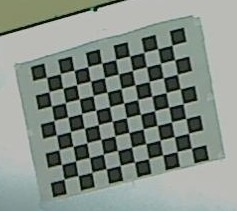
\includegraphics[width=3cm,height=3cm]{../Thesis_work/Latex_thesis_work/img_source/cam_1.png}} &  
\hspace{-0.3cm}\subfloat[]{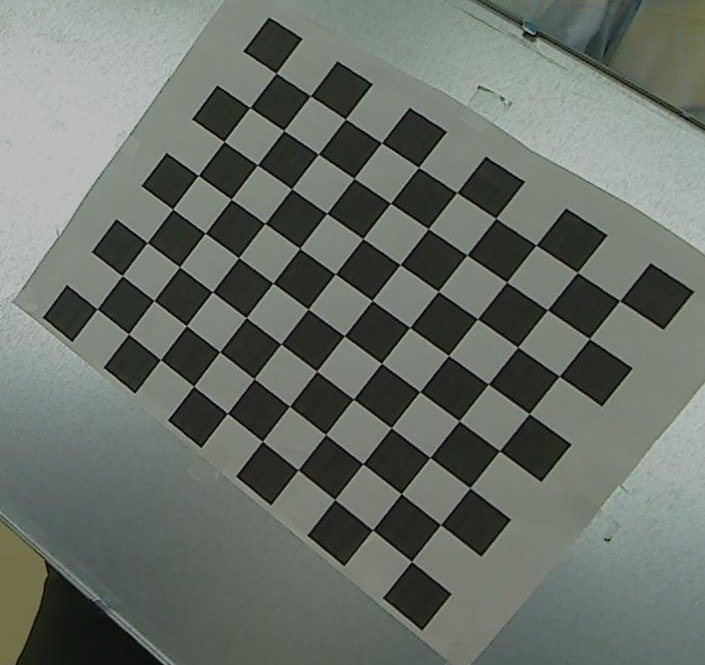
\includegraphics[width=3cm,height=3cm]{../Thesis_work/Latex_thesis_work/img_source/cam_2.png}} &  
\hspace{-0.3cm}\subfloat[]{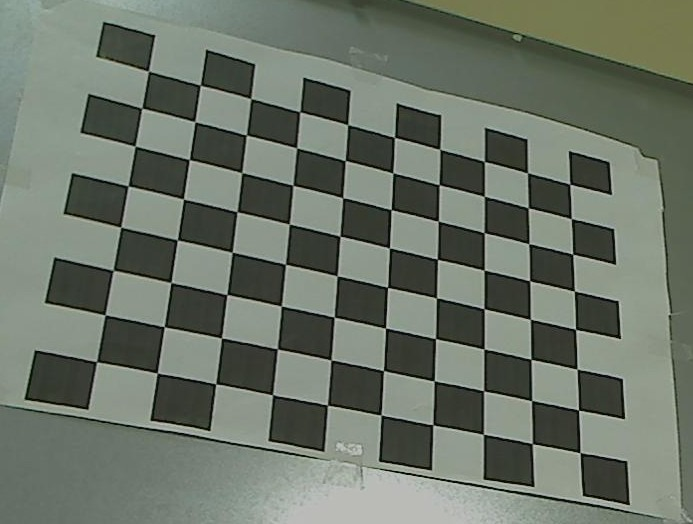
\includegraphics[width=3cm,height=3cm]{../Thesis_work/Latex_thesis_work/img_source/cam_3.png}} &  
\hspace{-0.3cm}\subfloat[]{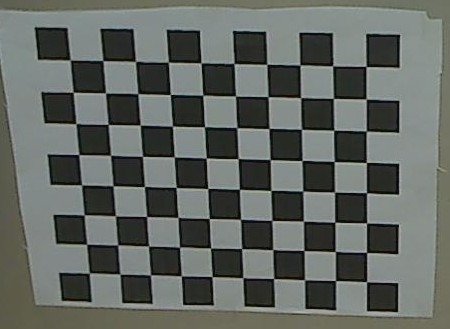
\includegraphics[width=3cm,height=3cm]{../Thesis_work/Latex_thesis_work/img_source/cam_4.png}}\\  
\end{tabular}  
\end{tabularx}  
\caption{Some views used for camera calibration}  
\label{fig:cam_calib_views}
\end{figure}  
\vspace{-0.5cm}
\begin{table}[ht]  
\centering  
\begin{tabular}{c l}  
\hline\noalign{\smallskip}  
Parameter & Estimated value \\  
\noalign{\smallskip}\hline\noalign{\smallskip}  
$f_x$ & 1362.152\\  
$f_y$ & 1372.189\\  
$c_x$ & 803.884\\  
$c_y$ & 590.066\\  
$k_1$ & 0.073\\  
$k_2$ & -0.143\\   
Reprojection error & 0.195 \\  
\noalign{\smallskip}\hline  
\end{tabular}  
\caption{Estimated Camera intrinsic model parameters}  
\end{table}  
\end{frame}
%%%%%%%%%%%%%%%%%%%%%%%%%%%%%%%%%%%%%%%%%%%%%%%%%%%%%%%%%%%%%%%%%%%%%%%%%%%%SLIDE ENDS%%%%%%%%%%%%%%%%%%%%%%%%%%%%%%%%%%%%%%%

%%%%%%%%%%%%%%%%%%%%%%%%%%%%%%%%%%%%%%%%%%%%%%%%%%%%%%%%%%%%%%%%%%%%%%%%%%%%%SLIDE starts%%%%%%%%%%%%%%%%%%%%%%%%%%%%%%%%%%%%%
\begin{frame}
SciLab script was developed to visualize calibration results for camera and projector calibration.
\begin{figure} 
\begin{tabularx}{\linewidth}{@{}cXX@{}}
\begin{tabular}{l r}
\subfloat[View along X-axis]{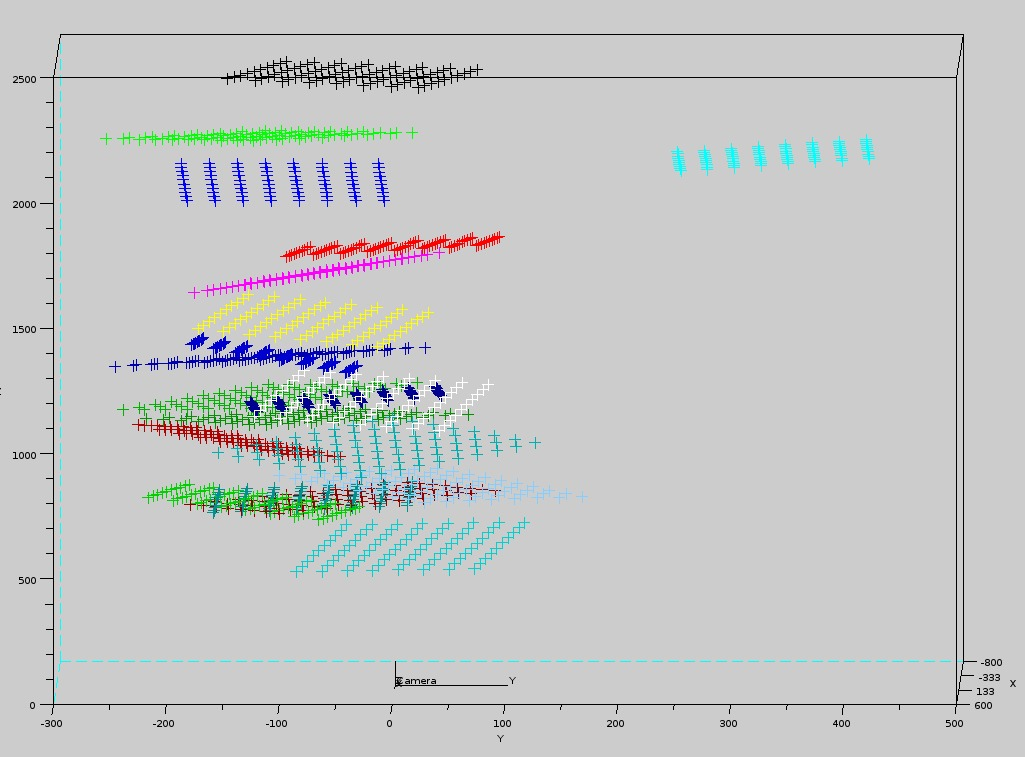
\includegraphics[width=6cm,height=6cm]{../Thesis_work/Latex_thesis_work/img_source/cam_calib_view.png}} &  
\hspace{-0.3cm}\subfloat[View along Y-axis]{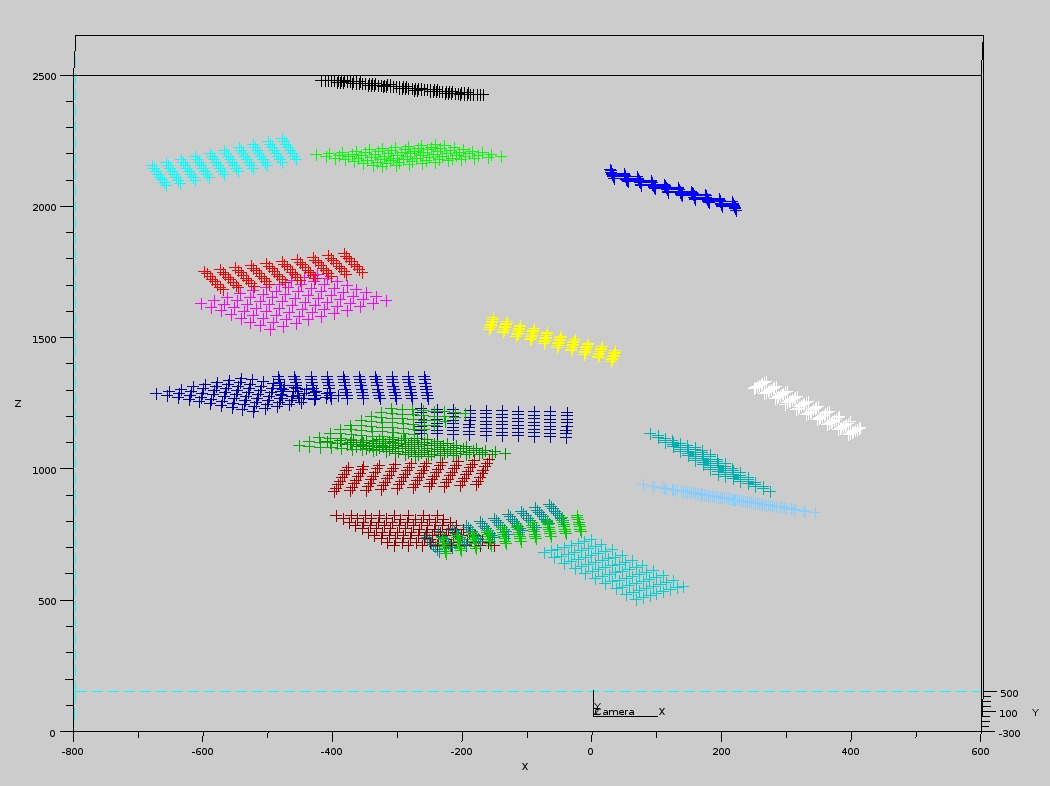
\includegraphics[width=6cm,height=6cm]{../Thesis_work/Latex_thesis_work/img_source/cam_calib_view2.png}} \\  
\end{tabular}
\end{tabularx} 
\caption{Visualization of camera calibration results} 
\end{figure}  
\end{frame}
%%%%%%%%%%%%%%%%%%%%%%%%%%%%%%%%%%%%%%%%%%%%%%%%%%%%%%%%%%%%%%%%%%%%%%%%%%%%SLIDE ENDS%%%%%%%%%%%%%%%%%%%%%%%%%%%%%%%%%%%%%%%

%%%%%%%%%%%%%%%%%%%%%%%%%%%%%%%%%%%%%%%%%%%%%%%%%%%%%%%%%%%%%%%%%%%%%%%%%%%%%SLIDE starts%%%%%%%%%%%%%%%%%%%%%%%%%%%%%%%%%%%%%
\begin{frame}
\frametitle{Projector calibration}
\begin{enumerate}
\item Projector assumed as \textit{inverse camera}.
\item Camera used as a feedback device which will provide the 3D coordinates for the 2D features projected by the projector.
\end{enumerate}
\begin{figure}[h!]  
%\def\tabularxcolumn#1{m{#1}}  
\begin{tabularx}{\linewidth}{@{}cXX@{}}  
\begin{tabular}{c c c c}   
\hspace{-0.3cm}\subfloat[]{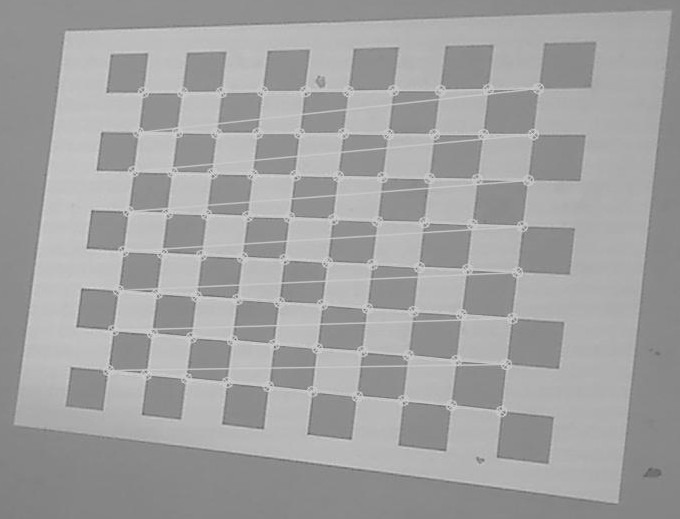
\includegraphics[width=3cm,height=3cm]{../Thesis_work/Latex_thesis_work/img_source/proj_view_1.png}} &  
\hspace{-0.3cm}\subfloat[]{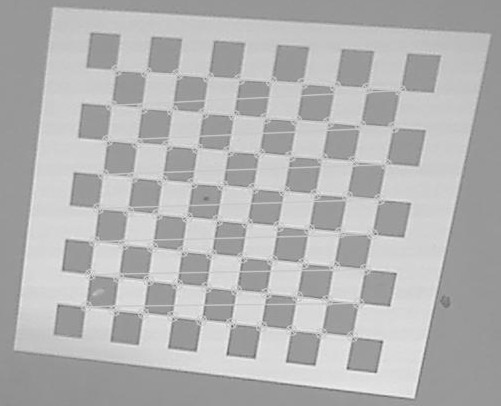
\includegraphics[width=3cm,height=3cm]{../Thesis_work/Latex_thesis_work/img_source/proj_view_2.png}} &  
\hspace{-0.3cm}\subfloat[]{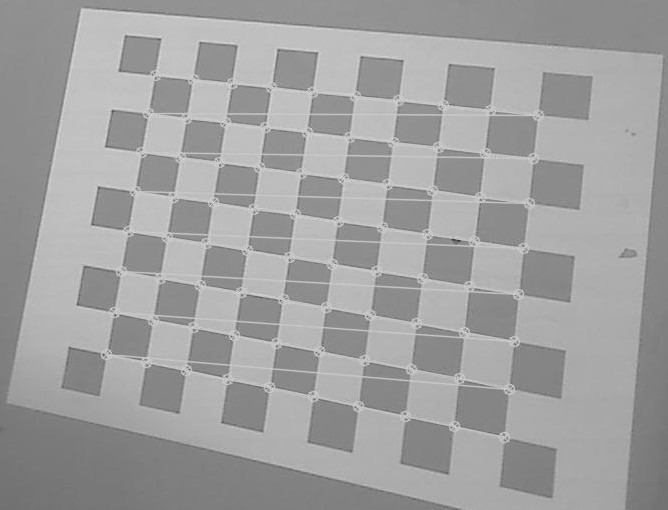
\includegraphics[width=3cm,height=3cm]{../Thesis_work/Latex_thesis_work/img_source/proj_view_3.png}} &  
\hspace{-0.3cm}\subfloat[]{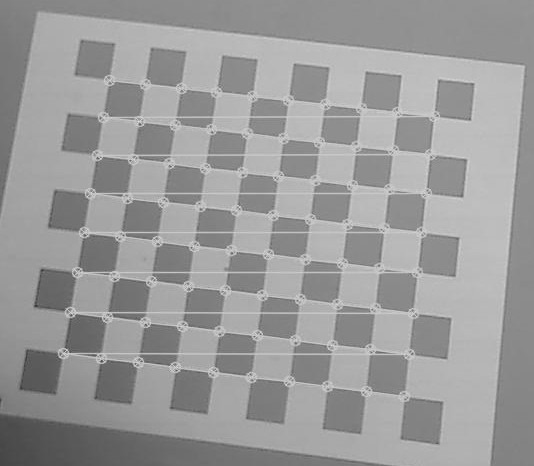
\includegraphics[width=3cm,height=3cm]{../Thesis_work/Latex_thesis_work/img_source/proj_view_4.png}} \\  
\end{tabular}  
\end{tabularx}  
\caption{Some view used for projector calibration} 
\label{fig:proj_calib_view} 
\end{figure} 
\vspace{-0.6cm}
\begin{table}[h]  
\centering  
\begin{tabular}{c l}  
\hline\noalign{\smallskip}  
Parameter & Estimated value \\  
\noalign{\smallskip}\hline\noalign{\smallskip}  
$f_x$ & 2261.710\\  
$f_y$ & 2262.799\\  
$c_x$ & 522.666\\  
$c_y$ & 713.840\\  
\noalign{\smallskip}\hline  
\end{tabular}  
\caption{Estimated Projector intrinsic model parameters}  
\end{table}  
\end{frame}
%%%%%%%%%%%%%%%%%%%%%%%%%%%%%%%%%%%%%%%%%%%%%%%%%%%%%%%%%%%%%%%%%%%%%%%%%%%%SLIDE ENDS%%%%%%%%%%%%%%%%%%%%%%%%%%%%%%%%%%%%%%%


%%%%%%%%%%%%%%%%%%%%%%%%%%%%%%%%%%%%%%%%%%%%%%%%%%%%%%%%%%%%%%%%%%%%%%%%%%%%%SLIDE starts%%%%%%%%%%%%%%%%%%%%%%%%%%%%%%%%%%%%%
\begin{frame}
\begin{figure} 
\begin{tabularx}{\linewidth}{@{}cXX@{}}
\begin{tabular}{l r}
\hspace{-0.3cm}\subfloat[View along X-axis]{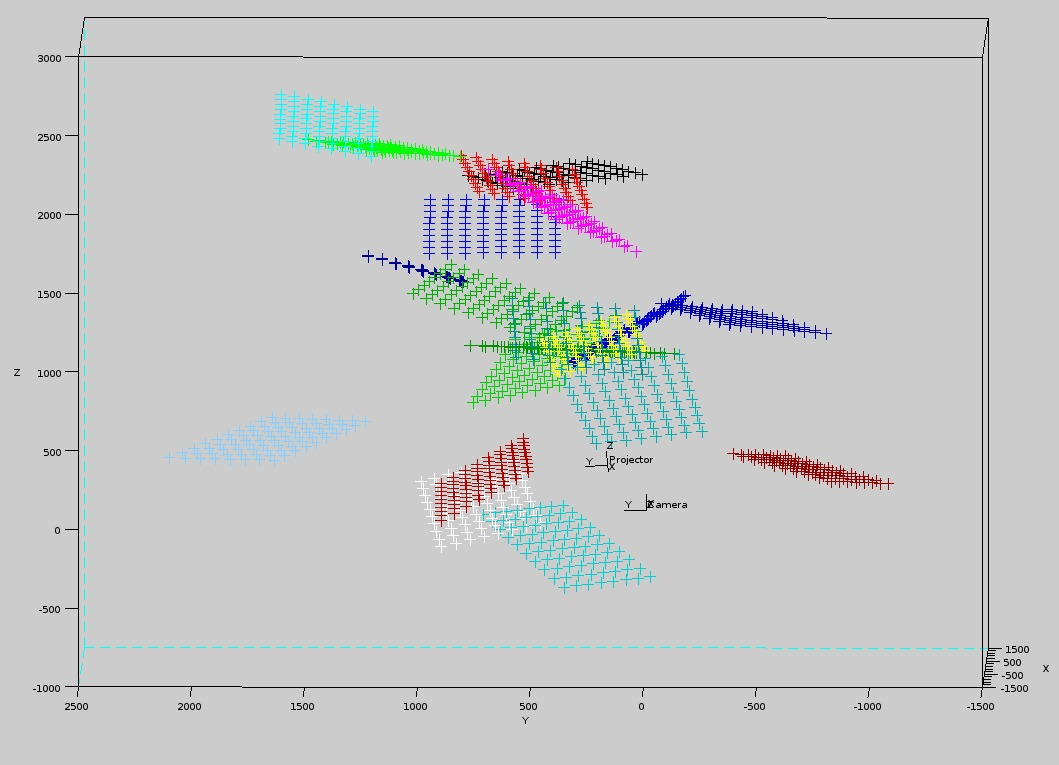
\includegraphics[width=6cm,height=6cm]{../Thesis_work/Latex_thesis_work/img_source/proj_calib_plot_2.png}} &
\subfloat[View along Y-axis]{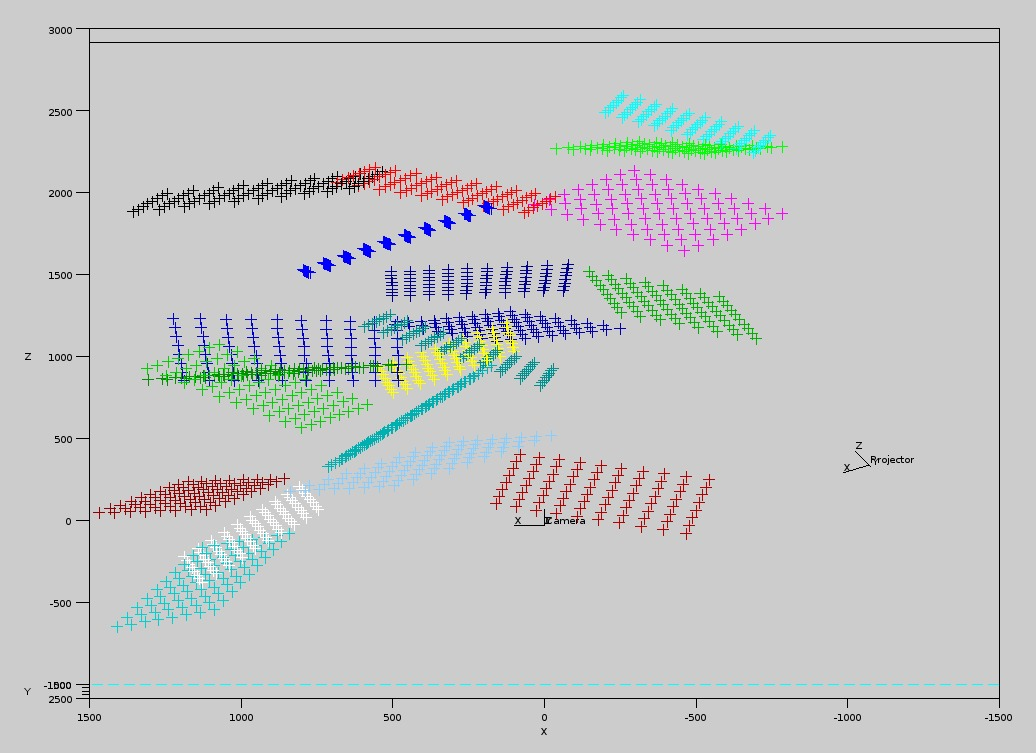
\includegraphics[width=6cm,height=6cm]{../Thesis_work/Latex_thesis_work/img_source/proj_calib_plot_1.png}} \\  
\end{tabular}
\end{tabularx} 
\caption{Visualization of projector calibration results} 
\end{figure}  
\end{frame}
%%%%%%%%%%%%%%%%%%%%%%%%%%%%%%%%%%%%%%%%%%%%%%%%%%%%%%%%%%%%%%%%%%%%%%%%%%%%SLIDE ENDS%%%%%%%%%%%%%%%%%%%%%%%%%%%%%%%%%%%%%%%

%%%%%%%%%%%%%%%%%%%%%%%%%%%%%%%%%%%%%%%%%%%%%%%%%%%%%%%%%%%%%%%%%%%%%%%%%%%%%SLIDE starts%%%%%%%%%%%%%%%%%%%%%%%%%%%%%%%%%%%%%
\begin{frame}
\frametitle{Projector-camera extrinsic calibration}
Estimating rotation and translation vectors for transforming a point in projector coordinate system to camera coordinate system.
\begin{equation}  
\begin{bmatrix}  
P_c \\  
P_p  
\end{bmatrix}  
=\begin{bmatrix}  
R_{wc}*P_w \\  
R_{wp}*P_w  
\end{bmatrix}  
+\begin{bmatrix}  
T_{wc} \\  
T_{wp}  
\end{bmatrix}  
\end{equation}  
hence,\newline  
$P_c=\underbrace{(R_c*R_p^{-1})}_{R_{pc}}*P_p+\underbrace{(T_c-R_c*R_p^{-1}*P_p)}_{T_{pc}}$  
\vspace{-0.5cm}
\begin{figure}
\begin{tabularx}{\linewidth}{@{}cXX@{}}  
\begin{tabular}{c c}
\subfloat[]{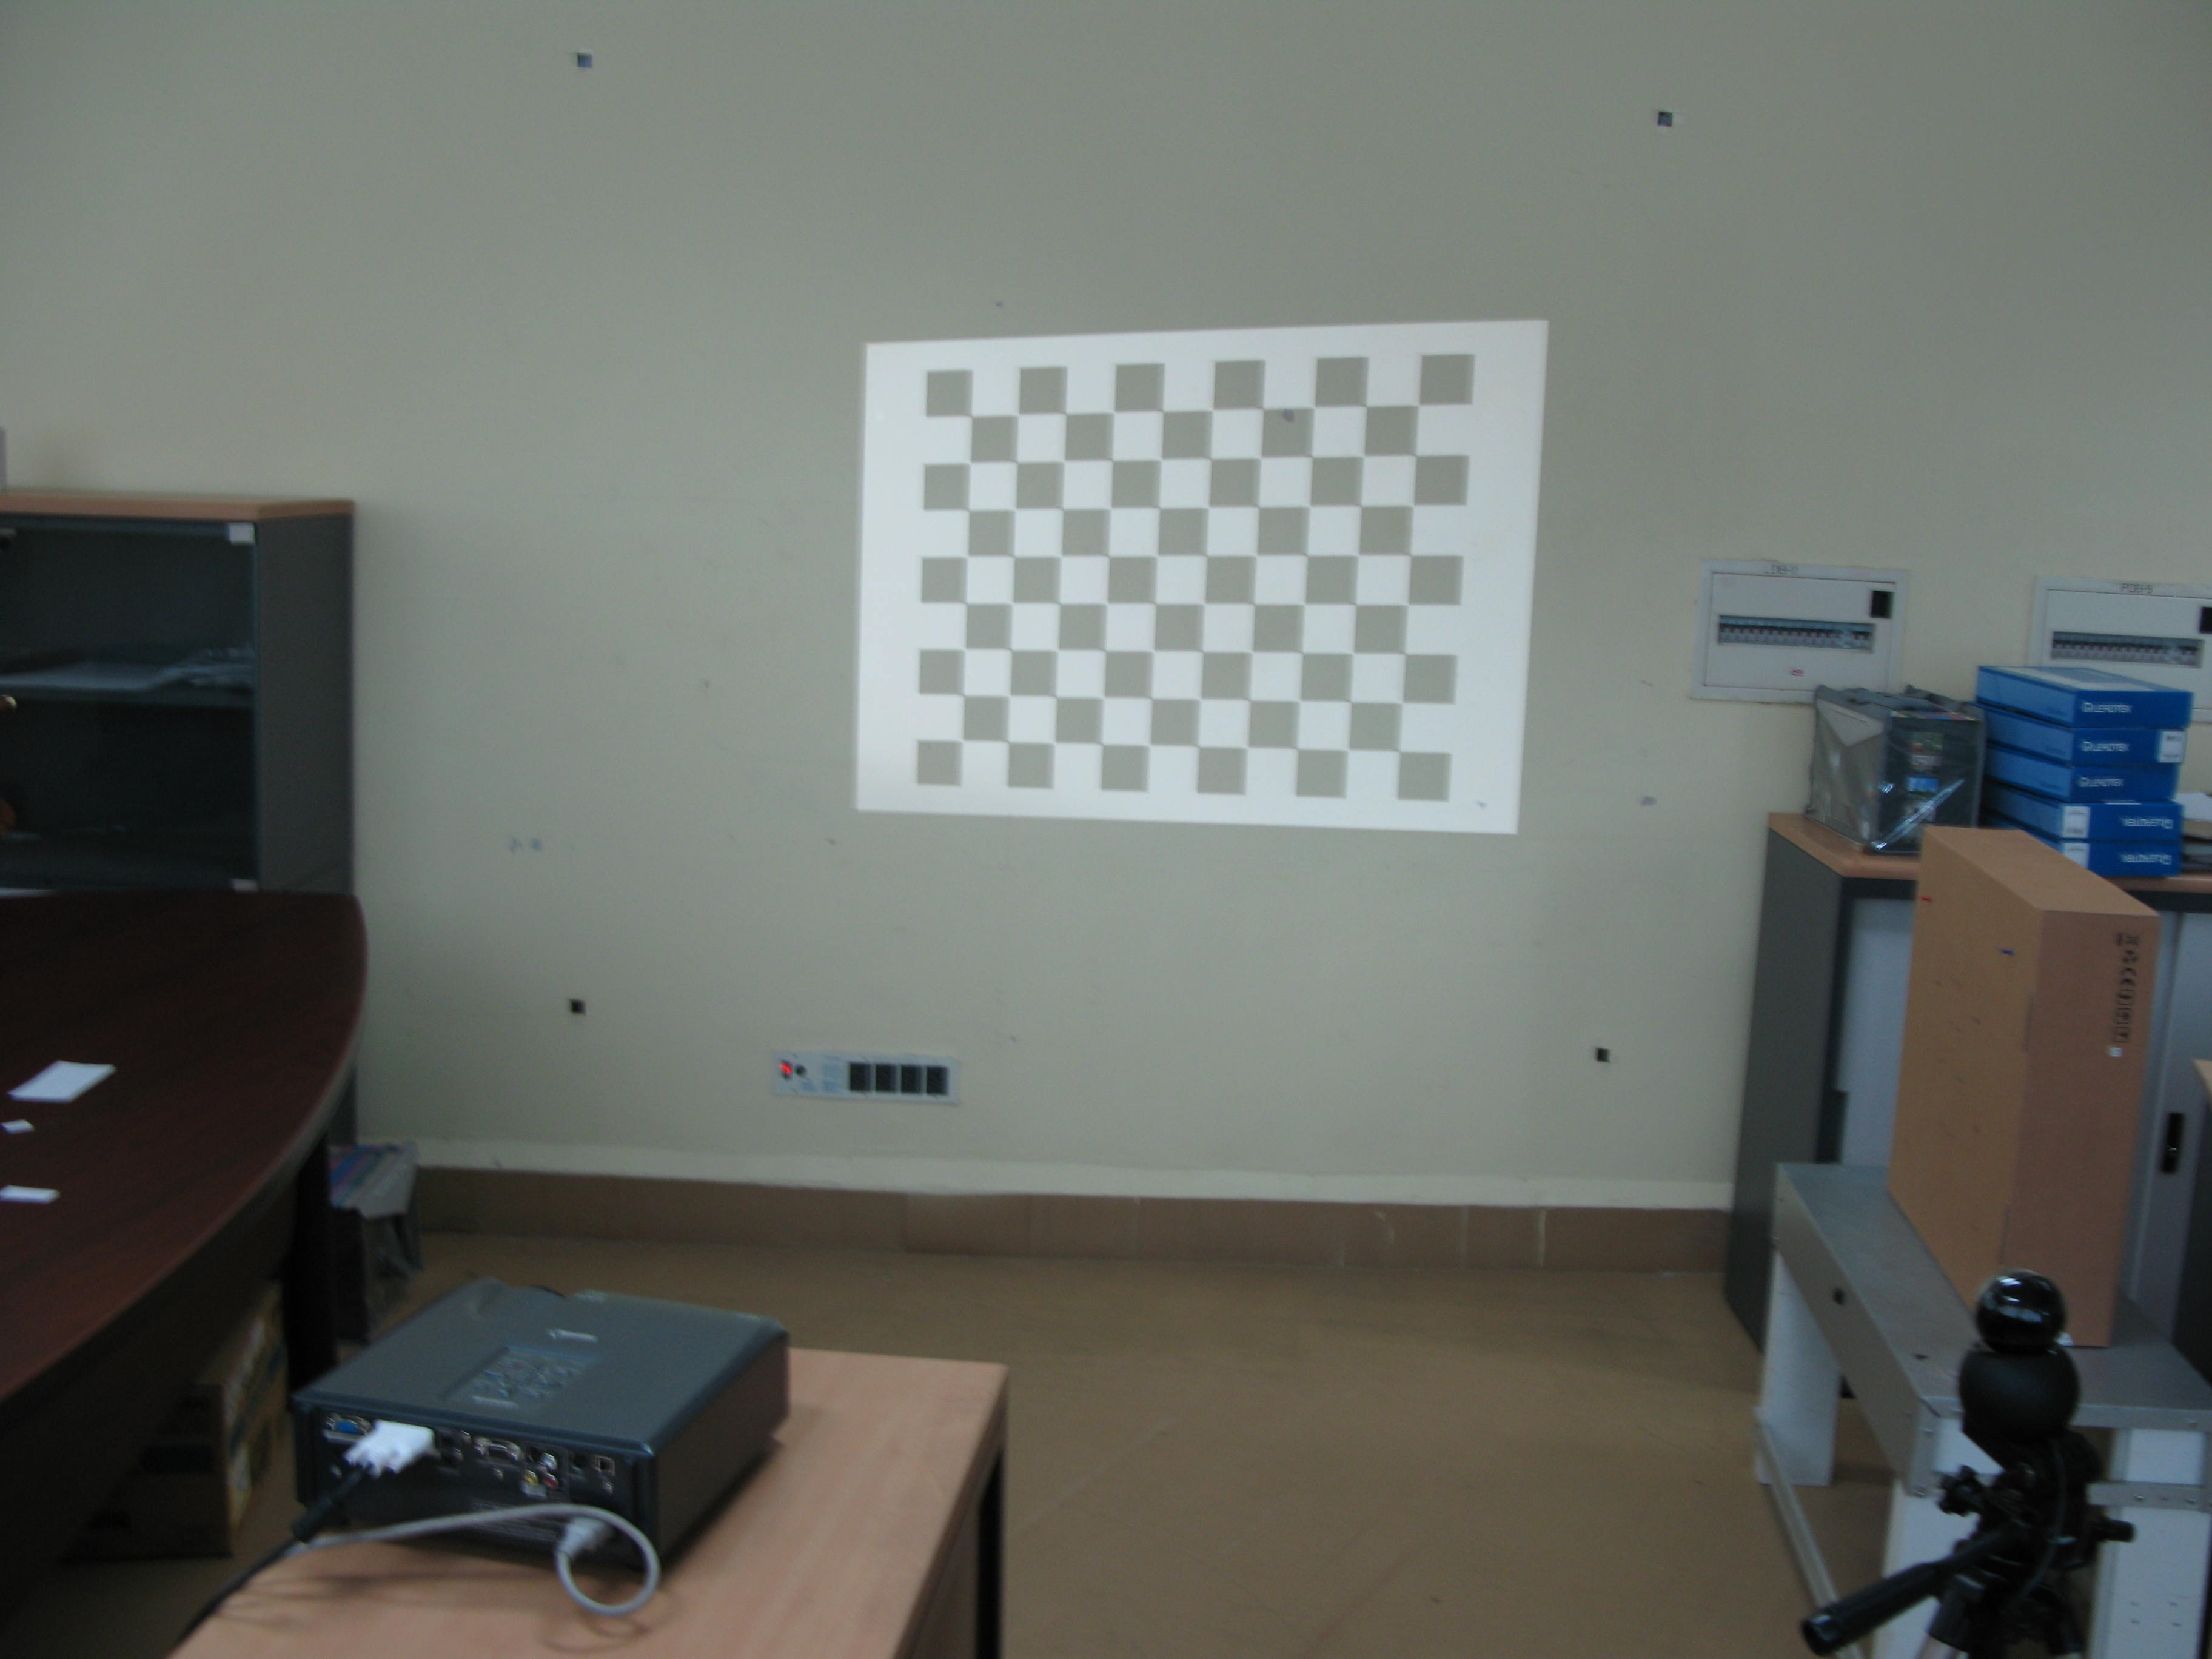
\includegraphics[width=5cm,height=5cm]{../Thesis_work/Latex_thesis_work/img_source/system_extrinsic.png}}  
\subfloat[]{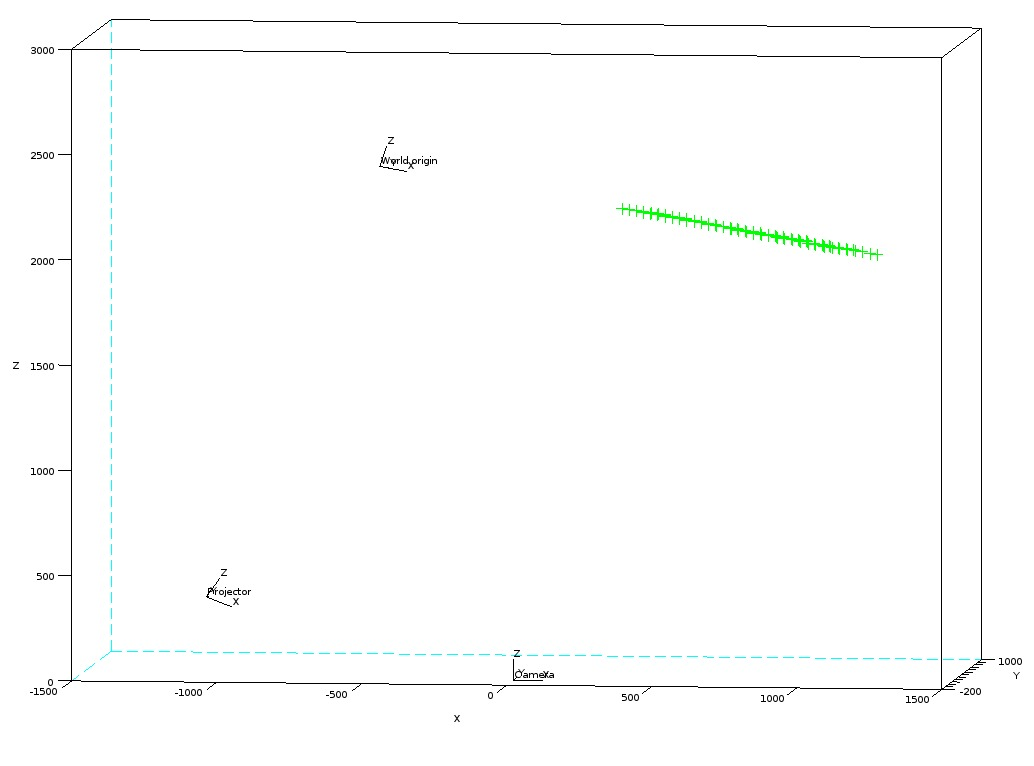
\includegraphics[width=7cm,height=5cm]{../Thesis_work/Latex_thesis_work/img_source/system_plot.png}}
\end{tabular}
\end{tabularx}
\label{fig:extrinsic_calib_setup}
\end{figure}  
\end{frame}
%%%%%%%%%%%%%%%%%%%%%%%%%%%%%%%%%%%%%%%%%%%%%%%%%%%%%%%%%%%%%%%%%%%%%%%%%%%%SLIDE ENDS%%%%%%%%%%%%%%%%%%%%%%%%%%%%%%%%%%%%%%%


%%%%%%%%%%%%%%%%%%%%%%%%%%%%%%%%%%%%%%%%%%%%%%%%%%%%%%%%%%%%%%%%%%%%%%%%%%%%%SLIDE starts%%%%%%%%%%%%%%%%%%%%%%%%%%%%%%%%%%%%%
\begin{frame}
\frametitle{Triangulation module}
To assign 3D coordinates to a point viewed by both camera and projector,\newline
For camera,
\begin{equation}
\begin{bmatrix}
w_c*u_i^c \\
w_c*v_i^c \\
w_c
\end{bmatrix}
=\begin{bmatrix}
a_{1,1}^c & a_{1,2}^c & a_{1,3}^c & a_{1,4}^c \\
a_{2,1}^c & a_{2,2}^c & a_{2,3}^c & a_{2,4}^c \\
a_{3,1}^c & a_{3,2}^c & a_{3,3}^c & a_{3,4}^c 
\end{bmatrix}
\begin{bmatrix}
x_i^w\\
y_i^w\\
z_i^w\\
1
\end{bmatrix}
\end{equation}
Similarly,for projector,
\begin{equation}
\begin{bmatrix}
w_c*u_i^p \\
w_c*v_i^p \\
w_p
\end{bmatrix}
=\begin{bmatrix}
a_{1,1}^p & a_{1,2}^p & a_{1,3}^p & a_{1,4}^p \\
a_{2,1}^p & a_{2,2}^p & a_{2,3}^p & a_{2,4}^p \\
a_{3,1}^p & a_{3,2}^p & a_{3,3}^p & a_{3,4}^p 
\end{bmatrix}
\begin{bmatrix}
x_i^w\\
y_i^w\\
z_i^w\\
1
\end{bmatrix}
\end{equation}
In matrix form it can be written as,
\begin{equation}
PV=F
\end{equation}
\noindent
where,\newline
\newline
P=$\begin{bmatrix}
(a_{1,1}^c-u_i^ca_{3,1}^c) & (a_{1,2}^c-u_i^ca_{3,2}^c) & (a_{1,3}^c-u_i^ca_{3,3}^c) \\ (a_{2,1}^c-v_i^ca_{3,1}^c) & (a_{2,2}^c-v_i^ca_{3,2}^c) & (a_{2,3}^c-v_i^ca_{3,3}^c) \\
(a_{1,1}^p-u_i^pa_{3,1}^p) & (a_{1,2}^p-u_i^pa_{3,2}^p) & (a_{1,3}^p-u_i^pa_{3,3}^p) \\ (a_{2,1}^p-v_i^pa_{3,1}^p) & (a_{2,2}^p-v_i^pa_{3,2}^p) & (a_{2,3}^p-v_i^pa_{3,3}^p)
\end{bmatrix},V=\begin{bmatrix}
x_i^w\\
y_i^w\\
z_i^w
\end{bmatrix},F=\begin{bmatrix}
a_{3,4}^cu_i^c-a_{1,4}^c\\
a_{3,4}^cv_i^c-a_{2,4}^c\\
a_{3,4}^pu_i^p-a_{1,4}^p\\
a_{3,4}^pv_i^p-a_{2,4}^p
\end{bmatrix}$\newline 
\end{frame}
%%%%%%%%%%%%%%%%%%%%%%%%%%%%%%%%%%%%%%%%%%%%%%%%%%%%%%%%%%%%%%%%%%%%%%%%%%%%SLIDE ENDS%%%%%%%%%%%%%%%%%%%%%%%%%%%%%%%%%%%%%%%

%%%%%%%%%%%%%%%%%%%%%%%%%%%%%%%%%%%%%%%%%%%%%%%%%%%%%%%%%%%%%%%%%%%%%%%%%%%%%SLIDE starts%%%%%%%%%%%%%%%%%%%%%%%%%%%%%%%%%%%%%
\begin{frame}
Results of applying equation $PV=F$,
\begin{figure}
%\def\tabularxcolumn#1{m{#1}}
\begin{tabularx}{\linewidth}{@{}cXX@{}}
\begin{tabular}{c c c c}
\hspace{-0.3cm}\subfloat[2D face image]{\includegraphics[width=3cm,height=3cm]{../Thesis_work/Latex_thesis_work/img_source/face_2d.png}} & 
\hspace{-0.3cm}\subfloat[3D reconstruction of face]{\includegraphics[width=3cm,height=3cm]{../Thesis_work/Latex_thesis_work/img_source/face_3d.png}} &
\hspace{-0.3cm}\subfloat[2D image of box in front of wall]{\includegraphics[width=3cm,height=3cm]{../Thesis_work/Latex_thesis_work/img_source/box_wall_2d.png}} & 
\hspace{-0.3cm}\subfloat[3D reconstruction of box in front of wall]{\includegraphics[width=3cm,height=3cm]{../Thesis_work/Latex_thesis_work/img_source/box_wall_3d.png}}\\
\hspace{-0.3cm}\subfloat[2D image of a chair with background]{\includegraphics[width=3cm,height=3cm]{../Thesis_work/Latex_thesis_work/img_source/chair_2d.png}} &
\hspace{-0.3cm}\subfloat[3D reconstruction of chair with background]{\includegraphics[width=3cm,height=3cm]{../Thesis_work/Latex_thesis_work/img_source/chair_reconstruction.png}} &
\hspace{-0.3cm}\subfloat[A cup]{\includegraphics[width=3cm,height=3cm]{../Thesis_work/Latex_thesis_work/img_source/cup_2d.png}} &
\hspace{-0.3cm}\subfloat[3D reconstruction of cup]{\includegraphics[width=3cm,height=3cm]{../Thesis_work/Latex_thesis_work/img_source/cup_3d.png}}\\ 
\end{tabular}
\end{tabularx}
\caption{Some 3D reconstruction results}
\end{figure}
\end{frame}
%%%%%%%%%%%%%%%%%%%%%%%%%%%%%%%%%%%%%%%%%%%%%%%%%%%%%%%%%%%%%%%%%%%%%%%%%%%%SLIDE ENDS%%%%%%%%%%%%%%%%%%%%%%%%%%%%%%%%%%%%%%%
%%%%%%%%%%%%%%%%%%%%%%%%%%%%%%%%%%%%%%%%%%%%%%%%%%%%%%%%%%%%%%%%%%%%%%%%%%%%%SLIDE starts%%%%%%%%%%%%%%%%%%%%%%%%%%%%%%%%%%%%%
\begin{frame}
\frametitle{Accuracy analysis:System calibration}
Goal was to assess \textit{repeatability} and \textit{accuracy} of estimated calibration parameters.
\begin{enumerate}
\item Repeatability was judged based on repeatedly performing camera and projector calibration and determining the \% deviation of individual estimated parameters from their \textit{mean} values.
\item The definition of \textit{system calibration error} $\varepsilon$ used in this work:
\begin{equation}
\varepsilon=\frac{\sum_{i=1}^N\sqrt[2]{(X_t^i-X_e^i)^2+(Y_t^i-Y_e^i)^2}}{N}
\end{equation}
\end{enumerate}
\end{frame}
%%%%%%%%%%%%%%%%%%%%%%%%%%%%%%%%%%%%%%%%%%%%%%%%%%%%%%%%%%%%%%%%%%%%%%%%%%%%SLIDE ENDS%%%%%%%%%%%%%%%%%%%%%%%%%%%%%%%%%%%%%%%

%%%%%%%%%%%%%%%%%%%%%%%%%%%%%%%%%%%%%%%%%%%%%%%%%%%%%%%%%%%%%%%%%%%%%%%%%%%%%SLIDE starts%%%%%%%%%%%%%%%%%%%%%%%%%%%%%%%%%%%%%
\begin{frame}
\frametitle{Camera calibration:Repeatability}
OpenCV method was used for camera calibration.
\begin{table}[ht]
\centering
\begin{tabular}{c c}
\hline\noalign{\smallskip}
Parameter  & \% deviation \\
\noalign{\smallskip}\hline\noalign{\smallskip}
$f_x$   & 1.105  \\
$f_y$   & 1.075  \\
$c_x$   & 0.707  \\
$c_y$   & 0.894  \\
$k_1$   & 7.357 \\
$k_2$  &  8.825 \\
\noalign{\smallskip}\hline
\end{tabular}
\caption{Percentage average absolute deviation of camera calibration parameters}
\end{table}

Comparatively high deviation in $k_1$ and $k_2$ observed.\newline
Possibly due to use of lenses with very low/negligible \textit{radial} distortion. 
\end{frame}
%%%%%%%%%%%%%%%%%%%%%%%%%%%%%%%%%%%%%%%%%%%%%%%%%%%%%%%%%%%%%%%%%%%%%%%%%%%%SLIDE ENDS%%%%%%%%%%%%%%%%%%%%%%%%%%%%%%%%%%%%%%%

%%%%%%%%%%%%%%%%%%%%%%%%%%%%%%%%%%%%%%%%%%%%%%%%%%%%%%%%%%%%%%%%%%%%%%%%%%%%%SLIDE starts%%%%%%%%%%%%%%%%%%%%%%%%%%%%%%%%%%%%%
\begin{frame}
\frametitle{Camera calibration:Accuracy}
\begin{figure}[ht]
\centering
\includegraphics[width=5cm,height=4.5cm]{../Thesis_work/Latex_thesis_work/img_source/camera_calib_test.jpg}
\caption{Points A,B,C,D were used for measuring camera calibration accuracy}
\label{fig:cam_calib_accuracy}
\end{figure}
\begin{table}[ht]
\centering
\vspace{-0.4cm}\begin{tabular}{c c}
\hline\noalign{\smallskip}
Point  & Radial distance from true projection \\
\noalign{\smallskip}\hline\noalign{\smallskip}
A   & 2.553  \\
B   & 3.453  \\
C   & 4.080 \\
D   & 4.180 \\
\noalign{\smallskip}\hline
\end{tabular}
\caption{Camera calibration:Radial error of projection}
\end{table}
\end{frame}
%%%%%%%%%%%%%%%%%%%%%%%%%%%%%%%%%%%%%%%%%%%%%%%%%%%%%%%%%%%%%%%%%%%%%%%%%%%%SLIDE ENDS%%%%%%%%%%%%%%%%%%%%%%%%%%%%%%%%%%%%%%%

%%%%%%%%%%%%%%%%%%%%%%%%%%%%%%%%%%%%%%%%%%%%%%%%%%%%%%%%%%%%%%%%%%%%%%%%%%%%%SLIDE starts%%%%%%%%%%%%%%%%%%%%%%%%%%%%%%%%%%%%%
\begin{frame}
\frametitle{Projector calibration:Repeatability}
Experimented with OpenCV calibration algorithm and VPCLib algorithm.
\begin{table}[ht]
\centering
\begin{tabular}{c c c}
\hline\noalign{\smallskip}
Parameter  & OpenCV method & VPCLib method \\
\noalign{\smallskip}\hline\noalign{\smallskip}
$f_x$ & 7.625 & 2.166\\
$f_y$ & 7.445 & 2.047\\
$c_x$ & 5.559 & 1.795\\
$c_y$ & 4.381 & 1.861\\
$k_1$ & 38.196 & Not estimated\\
$k_2$ & 96.227 & Not estimated\\
\noalign{\smallskip}\hline
\end{tabular}
\caption{Percentage average absolute deviation of projector calibration parameters}
\end{table}
Very high values for $k_1$,$k_2$ may be due to the fact that projectors generally have negligible lens distortions.\newline
VPCLib method gives higher repeatability as compared to OpenCV for projector calibration.Hence it was used in further work.
\end{frame}
%%%%%%%%%%%%%%%%%%%%%%%%%%%%%%%%%%%%%%%%%%%%%%%%%%%%%%%%%%%%%%%%%%%%%%%%%%%%SLIDE ENDS%%%%%%%%%%%%%%%%%%%%%%%%%%%%%%%%%%%%%%%

%%%%%%%%%%%%%%%%%%%%%%%%%%%%%%%%%%%%%%%%%%%%%%%%%%%%%%%%%%%%%%%%%%%%%%%%%%%%%SLIDE starts%%%%%%%%%%%%%%%%%%%%%%%%%%%%%%%%%%%%%
\begin{frame}
\frametitle{Projector calibration:Accuracy}
\begin{figure}
\centering
\includegraphics[width=5cm,height=4.5cm]{../Thesis_work/Latex_thesis_work/img_source/proj_calib_test.jpg}
\caption{Corners A,B,C,D were used for assessing accuracy of projector calibration parameters}
\label{fig:proj_calib_accuracy}
\end{figure}

\begin{table}[ht]
\centering
\vspace{-0.4cm}\begin{tabular}{c c}
\hline\noalign{\smallskip}
Point  & Radial distance from true projection \\
\noalign{\smallskip}\hline\noalign{\smallskip}
A   &  6.776 \\
B   &  8.608 \\
C   &  11.728\\
D   &  18.248\\
\noalign{\smallskip}\hline
\end{tabular}
\caption{Projector calibration:Radial error of projection}
\end{table}
\end{frame}
%%%%%%%%%%%%%%%%%%%%%%%%%%%%%%%%%%%%%%%%%%%%%%%%%%%%%%%%%%%%%%%%%%%%%%%%%%%%SLIDE ENDS%%%%%%%%%%%%%%%%%%%%%%%%%%%%%%%%%%%%%%%

%%%%%%%%%%%%%%%%%%%%%%%%%%%%%%%%%%%%%%%%%%%%%%%%%%%%%%%%%%%%%%%%%%%%%%%%%%%%%SLIDE starts%%%%%%%%%%%%%%%%%%%%%%%%%%%%%%%%%%%%%
%\begin{frame}
%\frametitle{Drawbacks \& limitations of the used evaluation approach}
%\begin{enumerate}
%\item Requires actual value of \textit{true} 3D reference coordinates which is not practical at larger distances from reference origin.
%\item For exhaustive testing at distance where true 3D coordinates can be conveniently measured,this approach is very time consuming.
%\item To define actual image points feature detector should be used which further adds error.
%\end{enumerate}
%\end{frame}
%%%%%%%%%%%%%%%%%%%%%%%%%%%%%%%%%%%%%%%%%%%%%%%%%%%%%%%%%%%%%%%%%%%%%%%%%%%%SLIDE ENDS%%%%%%%%%%%%%%%%%%%%%%%%%%%%%%%%%%%%%%%

%%%%%%%%%%%%%%%%%%%%%%%%%%%%%%%%%%%%%%%%%%%%%%%%%%%%%%%%%%%%%%%%%%%%%%%%%%%%%SLIDE starts%%%%%%%%%%%%%%%%%%%%%%%%%%%%%%%%%%%%%
\begin{frame}
\frametitle{Accuracy analysis:Stereo-correspondence}
Goal is to study the effect of non-linearities of input-output response of projector on estimated stereo-correspondence.\newline
Specifically,the effect of projector gamma in a 3 phase-shifted pattern system on accuracy of stereo-correspondence was studied.
\end{frame}
%%%%%%%%%%%%%%%%%%%%%%%%%%%%%%%%%%%%%%%%%%%%%%%%%%%%%%%%%%%%%%%%%%%%%%%%%%%%SLIDE ENDS%%%%%%%%%%%%%%%%%%%%%%%%%%%%%%%%%%%%%%%

%%%%%%%%%%%%%%%%%%%%%%%%%%%%%%%%%%%%%%%%%%%%%%%%%%%%%%%%%%%%%%%%%%%%%%%%%%%%%SLIDE starts%%%%%%%%%%%%%%%%%%%%%%%%%%%%%%%%%%%%%
\begin{frame}
\frametitle{Procedure}
A new approach for estimating error in stereo-matching was used in this work:
\begin{enumerate}
\item \textit{Known} checkerboard pattern was projected. 
\item Corners of checkerboard were detected and corresponding projector coordinates were determined using the estimated stereo-correspondence . 
\item Stereo-correspondence error $\varepsilon$ is defined to be the \textit{radial} distance of estimated projector coordinates for detected checkerboard corners from the actual coordinates of the checkerboard corners in projector image. 
\end{enumerate}

\begin{equation}
\varepsilon=\frac{\sum_{i=1}^N\sqrt[2]{(X_t^i-X_e^i)^2+(Y_t^i-Y_e^i)^2}}{N}
\end{equation}

\end{frame}
%%%%%%%%%%%%%%%%%%%%%%%%%%%%%%%%%%%%%%%%%%%%%%%%%%%%%%%%%%%%%%%%%%%%%%%%%%%%SLIDE ENDS%%%%%%%%%%%%%%%%%%%%%%%%%%%%%%%%%%%%%%%

%%%%%%%%%%%%%%%%%%%%%%%%%%%%%%%%%%%%%%%%%%%%%%%%%%%%%%%%%%%%%%%%%%%%%%%%%%%%%SLIDE starts%%%%%%%%%%%%%%%%%%%%%%%%%%%%%%%%%%%%%
\begin{frame}
\frametitle{Effect of projector gamma on 3D reconstruction}
\begin{figure}[h]
\vspace{0.5cm}
\begin{tabularx}{\linewidth}{@{}cXX@{}}
\begin{tabular}{c}
\hspace{1cm}\subfloat[$\gamma=1.0$]{\includegraphics[width=10cm,height=3cm]{../Thesis_work/Latex_thesis_work/img_source/3_phase_1.png}} \\ 
\hspace{1cm}\subfloat[$\gamma=2.041$]{\includegraphics[width=10cm,height=3cm]{../Thesis_work/Latex_thesis_work/img_source/3_phase_2_041.png}}\\
\end{tabular}
\end{tabularx}
\caption{Effect of gamma on 3D reconstruction of a plane}
\label{fig:gamma_3_phase}
\end{figure}
\end{frame}
%%%%%%%%%%%%%%%%%%%%%%%%%%%%%%%%%%%%%%%%%%%%%%%%%%%%%%%%%%%%%%%%%%%%%%%%%%%%SLIDE ENDS%%%%%%%%%%%%%%%%%%%%%%%%%%%%%%%%%%%%%%%

%%%%%%%%%%%%%%%%%%%%%%%%%%%%%%%%%%%%%%%%%%%%%%%%%%%%%%%%%%%%%%%%%%%%%%%%%%%%%SLIDE starts%%%%%%%%%%%%%%%%%%%%%%%%%%%%%%%%%%%%%
\begin{frame}
\frametitle{Experiment results}
\begin{table}[ht]
\caption{Stereo-correspondence error for various gamma values for 3 phase-shifted method}
\centering
\begin{tabular}{c c}
\hline\noalign{\smallskip}
Gamma($\gamma$)  & Stereo-correspondence error($\varepsilon$) \\
\noalign{\smallskip}\hline\noalign{\smallskip}
1.0   &  1.890\\
1.524   &  1.682 \\
1.912   &  1.730\\
2.041   &  1.588\\
2.559 & 2.073\\
2.947 & 2.394\\
\noalign{\smallskip}\hline
\end{tabular}
\end{table}
$\varepsilon$ decreases from $\gamma=1.0$ to $\gamma=2.041$ followed by increase from $\gamma=2.559$ onwards.
\end{frame}
%%%%%%%%%%%%%%%%%%%%%%%%%%%%%%%%%%%%%%%%%%%%%%%%%%%%%%%%%%%%%%%%%%%%%%%%%%%%SLIDE ENDS%%%%%%%%%%%%%%%%%%%%%%%%%%%%%%%%%%%%%%%

%%%%%%%%%%%%%%%%%%%%%%%%%%%%%%%%%%%%%%%%%%%%%%%%%%%%%%%%%%%%%%%%%%%%%%%%%%%%%SLIDE starts%%%%%%%%%%%%%%%%%%%%%%%%%%%%%%%%%%%%%
%\begin{frame}
%\frametitle{Effect of varying number of phase-shifted patterns}
%\begin{figure}[h]
%\begin{tabularx}{\linewidth}{@{}cXX@{}}
%\begin{tabular}{c}
%\hspace{1cm}\subfloat[3 phase]{\includegraphics[width=10cm,height=3cm]{../Thesis_work/Latex_thesis_work/img_source/phase_3.png}}\\ 
%\hspace{1cm}\vspace{0.3cm}\subfloat[4 phase]{\includegraphics[width=10cm,height=3cm]{../Thesis_work/Latex_thesis_work/img_source/phase_4.png}}
%\subfloat[5 phase]{\includegraphics[width=5cm,height=3cm]{../Thesis_work/Latex_thesis_work/img_source/phase_5.png}} \\
%\end{tabular}
%\end{tabularx}
%\caption{Effect of increasing number of phase shifted patterns on \textit{waviness} in 3D reconstruction}
%\label{fig:gamma_3_4_5}
%\end{figure}
%\end{frame}
%%%%%%%%%%%%%%%%%%%%%%%%%%%%%%%%%%%%%%%%%%%%%%%%%%%%%%%%%%%%%%%%%%%%%%%%%%%%SLIDE ENDS%%%%%%%%%%%%%%%%%%%%%%%%%%%%%%%%%%%%%%%

%%%%%%%%%%%%%%%%%%%%%%%%%%%%%%%%%%%%%%%%%%%%%%%%%%%%%%%%%%%%%%%%%%%%%%%%%%%%%SLIDE starts%%%%%%%%%%%%%%%%%%%%%%%%%%%%%%%%%%%%%
%\begin{frame}
%\frametitle{Results}

%Contradictory results obtained after performing experiments approximately 10 times.As shown in the table:
%\begin{table}[ht]
%\centering
%\begin{tabular}{c c}
%\hline\noalign{\smallskip}
%Number of patterns  & Stereo-correspondence error($\varepsilon$) \\
%\noalign{\smallskip}\hline\noalign{\smallskip}
%3   &  1.890 \\
%4   &  2.100 \\
%5   &  2.454\\
%\noalign{\smallskip}\hline
%\end{tabular}
%\caption{Stereo correspondence error for 3,4,5 phase shifted patterns}
%\end{table}

%Results show increase in $\varepsilon$ on increasing number of phase-shifted patterns.\newline
%Currently,analysis is in progress for this issue. 
%\end{frame}
%%%%%%%%%%%%%%%%%%%%%%%%%%%%%%%%%%%%%%%%%%%%%%%%%%%%%%%%%%%%%%%%%%%%%%%%%%%%SLIDE ENDS%%%%%%%%%%%%%%%%%%%%%%%%%%%%%%%%%%%%%%%

%%%%%%%%%%%%%%%%%%%%%%%%%%%%%%%%%%%%%%%%%%%%%%%%%%%%%%%%%%%%%%%%%%%%%%%%%%%%%SLIDE starts%%%%%%%%%%%%%%%%%%%%%%%%%%%%%%%%%%%%%
%\begin{frame}
%\frametitle{Drawbacks \& limitations of used evaluation approach}
%\begin{enumerate}
%\item This approach works as long as projected features can be \textit{uniquely} recognized i.e., explicit correspondence estimation for the reference pattern features itself is not required.
%\item Can be used in case of a planer scene with no occlusions,but not for all geometries in general.
%\item Accuracy of feature detection will also affect the computed stereo-correspondence error.
%\end{enumerate}
%\end{frame}
%%%%%%%%%%%%%%%%%%%%%%%%%%%%%%%%%%%%%%%%%%%%%%%%%%%%%%%%%%%%%%%%%%%%%%%%%%%%SLIDE ENDS%%%%%%%%%%%%%%%%%%%%%%%%%%%%%%%%%%%%%%%

%%%%%%%%%%%%%%%%%%%%%%%%%%%%%%%%%%%%%%%%%%%%%%%%%%%%%%%%%%%%%%%%%%%%%%%%%%%%%SLIDE starts%%%%%%%%%%%%%%%%%%%%%%%%%%%%%%%%%%%%%
\begin{frame}
\frametitle{Accuracy evaluation}
Goal is to study the effect of distance between measurement object and sensor on its \textit{precision} and \textit{measurement accuracy}.
\begin{equation}
Precision=\frac{\sum_{p=1}^{vp}\Big[\frac{\sum_{i=1}^{vs_{p}}\Big[\frac{mean_{p}-sample_{i}}{mean_{p}+1}\Big]}{vs_{p}}\Big]}{vp}
\end{equation}
\noindent
\begin{equation}
Accuracy=\frac{\sum_{i=1}^{N}\Big[\frac{Actual_{i}-measured_{i}}{Actual_{i}}\Big]}{N}
\end{equation}
In literature,
\begin{enumerate}
\item Deviation of scan data with respect to a 3D laser scan data has been considered as measurement error(Accurate laser calibration required),or
\item \textbf{VDI/VDE 2634} standard has been used as a reference for evaluating measurement accuracy and repeatability of optical instrument(Fabrication of highly accurate pyramidal structure of spheres required).
\end{enumerate}
\end{frame}
%%%%%%%%%%%%%%%%%%%%%%%%%%%%%%%%%%%%%%%%%%%%%%%%%%%%%%%%%%%%%%%%%%%%%%%%%%%%SLIDE ENDS%%%%%%%%%%%%%%%%%%%%%%%%%%%%%%%%%%%%%%%

%%%%%%%%%%%%%%%%%%%%%%%%%%%%%%%%%%%%%%%%%%%%%%%%%%%%%%%%%%%%%%%%%%%%%%%%%%%%%SLIDE starts%%%%%%%%%%%%%%%%%%%%%%%%%%%%%%%%%%%%%
\begin{frame}
\frametitle{Experiment procedure}
\underline{For assessing precision:}\newline
A plane was scanned 10 times for 5 depths varying from $\sim1.3m$ to $\sim2.5m$.Precision along X,Y,Z axes was calculated.\newline
\underline{For accuracy evaluation:}\newline
Distances AB,BC,CD,AD,AC,BD were measured with object at different distances varying from $\sim1.3m$ to $\sim2.5m$.
\begin{figure}
\includegraphics[width=6cm,height=5cm]{../Thesis_work/Latex_thesis_work/img_source/measurement_object.jpg}
\caption{Measurement object used in this work}
\end{figure}
\end{frame}
%%%%%%%%%%%%%%%%%%%%%%%%%%%%%%%%%%%%%%%%%%%%%%%%%%%%%%%%%%%%%%%%%%%%%%%%%%%%SLIDE ENDS%%%%%%%%%%%%%%%%%%%%%%%%%%%%%%%%%%%%%%%

%%%%%%%%%%%%%%%%%%%%%%%%%%%%%%%%%%%%%%%%%%%%%%%%%%%%%%%%%%%%%%%%%%%%%%%%%%%%%SLIDE starts%%%%%%%%%%%%%%%%%%%%%%%%%%%%%%%%%%%%%
\begin{frame}
\frametitle{Precision \& Accuracy:Coded phase shift scanner(CPSS)}
\begin{table}
% table caption is above the table
% table-1
\parbox{.45\linewidth}{
\caption{CPSS:Precision along X,Y,Z axes}
\begin{tabular}{c c c c}
\hline\noalign{\smallskip}
Distance & X\% & Y\% & Z\% \\
\noalign{\smallskip}\hline\noalign{\smallskip}
1.3 & 0.006418 & 0.009779 & 0.006695 \\
1.6 & 0.015143 &0.018461 & 0.036458\\
1.9 & 0.010009 & 0.024181&0.049911 \\
2.2 & 0.014109 & 0.028856 & 0.093916\\
2.5 & 0.009640 & 0.024728 & 0.140487 \\
\noalign{\smallskip}\hline
\end{tabular}
}
\end{table}
\begin{figure}[h]
\hspace{-1cm}
\begin{tikzpicture}
\begin{axis}[height=5cm,width=8cm,grid=major,xlabel=Distance,ylabel=\% deviation from mean,xmin=1.2,xmax=2.6,domain=1.2:2.6,legend entries={CPSS X-axis,CPSS Y-axis,CPSS Z-axis},legend pos=north west]
%X-AXIS
\addplot [red] coordinates {(1.3,0.006418) (1.6,0.015143) (1.9,0.010009) (2.2,0.014109) (2.5,0.009640)}; %node [pos=0.1,pin={-10:$X$},inner sep=0pt] {};

%Y-AXIS
\addplot [blue] coordinates {(1.3,0.009779) (1.6,0.018461) (1.9,0.024181) (2.2,0.028856) (2.5,0.024728)}; %node [pos=0.3,pin={-10:$Y$},inner sep=0pt] {};

%Z-AXIS
\addplot [green] coordinates {(1.3,0.006695) (1.6,0.036458) (1.9,0.049911) (2.2,0.093916) (2.5,0.140487)}; %node [pos=0.6,pin={-10:$Z$},inner sep=0pt] {};
\end{axis}
\end{tikzpicture}
\end{figure}

\end{frame}
%%%%%%%%%%%%%%%%%%%%%%%%%%%%%%%%%%%%%%%%%%%%%%%%%%%%%%%%%%%%%%%%%%%%%%%%%%%%SLIDE ENDS%%%%%%%%%%%%%%%%%%%%%%%%%%%%%%%%%%%%%%%

%%%%%%%%%%%%%%%%%%%%%%%%%%%%%%%%%%%%%%%%%%%%%%%%%%%%%%%%%%%%%%%%%%%%%%%%%%%%%SLIDE starts%%%%%%%%%%%%%%%%%%%%%%%%%%%%%%%%%%%%%
\begin{frame}
%table-2
\begin{table}
\parbox{.45\linewidth}{
\caption{CPSS:Dependence of measurement accuracy on distance}
\begin{tabular}{c c}
\hline\noalign{\smallskip}
Distance & CPSS(\% error) \\
\noalign{\smallskip}\hline\noalign{\smallskip}
1.3 & 1.153  \\
1.6 & 0.744    \\
1.9 & 1.393    \\
2.2 & 1.040    \\
2.5 & 0.758    \\
\noalign{\smallskip}\hline
\end{tabular}
}
%table-3
\parbox{.45\linewidth}{
\caption{CPSS:Dependence of measurement uncertainty on distance}
\begin{tabular}{c c}
\hline\noalign{\smallskip}
Distance  & CPSS(\% uncertainty) \\
\noalign{\smallskip}\hline\noalign{\smallskip}
1.3  & 0.095  \\
1.6  & 0.152   \\
1.9  & 0.433   \\
2.2 & 0.204  \\
2.5  & 0.134 \\
\noalign{\smallskip}\hline
\end{tabular}
}
\end{table}

\begin{figure}
\begin{tikzpicture}
\begin{axis}[height=5cm,width=8cm,grid=major,xlabel=Distance,ylabel=\% deviation from true value,xmin=1.2,xmax=2.7,domain=1.2:3.0,legend entries={CPSS,Kinect},legend pos=north east]
\addplot +[blue,error bars/.cd,y dir=both,y explicit] coordinates {
(1.3,1.153) +- (0.0,0.095)
(1.6,0.744) +- (0.0,0.152) 
(1.9,1.393) +- (0.0,0.433)
(2.2,1.040) +- (0.0,0.204)
(2.5,0.758) +- (0.0,0.134)
};
\end{axis}
\end{tikzpicture}
\end{figure}

\end{frame}
%%%%%%%%%%%%%%%%%%%%%%%%%%%%%%%%%%%%%%%%%%%%%%%%%%%%%%%%%%%%%%%%%%%%%%%%%%%%SLIDE ENDS%%%%%%%%%%%%%%%%%%%%%%%%%%%%%%%%%%%%%%%



%%%%%%%%%%%%%%%%%%%%%%%%%%%%%%%%%%%%%%%%%%%%%%%%%%%%%%%%%%%%%%%%%%%%%%%%%%%%%SLIDE starts%%%%%%%%%%%%%%%%%%%%%%%%%%%%%%%%%%%%%
\begin{frame}
\frametitle{Comparison with Microsoft \textit{Kinect}}
\underline{Kinect working principle}\newline
Estimates depth using disparity between reference position of a point in reference image and that in captured image. 
\begin{figure} 
\begin{tabularx}{\linewidth}{@{}cXX@{}}
\begin{tabular}{c c}
\hspace{1cm}\subfloat[Kinect]{\includegraphics[width=4cm,height=3cm]{../Thesis_work/Latex_thesis_work/img_source/kinect.png}} & 
\hspace{-0.3cm}\subfloat[Measurement principle]{\includegraphics[width=6cm,height=4cm]{../Thesis_work/Latex_thesis_work/img_source/kinect_measurement.png}} 
\end{tabular}
\end{tabularx}
\caption{Kinect operation principle}
\end{figure}
\begin{equation}
Z_k=\frac{Z_0}{1+\frac{Z_0d}{fb}}
\end{equation}

\end{frame}
%%%%%%%%%%%%%%%%%%%%%%%%%%%%%%%%%%%%%%%%%%%%%%%%%%%%%%%%%%%%%%%%%%%%%%%%%%%%SLIDE ENDS%%%%%%%%%%%%%%%%%%%%%%%%%%%%%%%%%%%%%%%

%%%%%%%%%%%%%%%%%%%%%%%%%%%%%%%%%%%%%%%%%%%%%%%%%%%%%%%%%%%%%%%%%%%%%%%%%%%%%SLIDE starts%%%%%%%%%%%%%%%%%%%%%%%%%%%%%%%%%%%%%
\begin{frame}
\begin{enumerate}
\item RGBDemo used for accessing \textit{raw} Kinect 3D data.Data from CPSS was also used without any processing.
\item MeshLab used for extracting region of interest from 3D dataset.
\item Point Cloud Library(PCL) used for 3D data visualization.
\end{enumerate}

\begin{figure}
\begin{tabularx}{\linewidth}{@{}cXX@{}}
\begin{tabular}{c c}
\hspace{3cm}\subfloat[RGB image]{\includegraphics[width=3cm,height=3cm]{../Thesis_work/Latex_thesis_work/img_source/kinect_rgb.png}} &
\hspace{-0.3cm}\subfloat[IR image]{\includegraphics[width=3cm,height=3cm]{../Thesis_work/Latex_thesis_work/img_source/kinect_ir.png}} \\
\hspace{3cm}\subfloat[Disparity map]{\includegraphics[width=3cm,height=3cm]{../Thesis_work/Latex_thesis_work/img_source/kinect_disparity.png}} &
\hspace{-0.3cm}\subfloat[3D point cloud]{\includegraphics[width=3cm,height=3cm]{../Thesis_work/Latex_thesis_work/img_source/kinect_point_cloud.png}}
\end{tabular}
\end{tabularx}
\caption{Kinect 3D reconstruction}
\end{figure}
\end{frame}
%%%%%%%%%%%%%%%%%%%%%%%%%%%%%%%%%%%%%%%%%%%%%%%%%%%%%%%%%%%%%%%%%%%%%%%%%%%%SLIDE ENDS%%%%%%%%%%%%%%%%%%%%%%%%%%%%%%%%%%%%%%%

%%%%%%%%%%%%%%%%%%%%%%%%%%%%%%%%%%%%%%%%%%%%%%%%%%%%%%%%%%%%%%%%%%%%%%%%%%%%%SLIDE starts%%%%%%%%%%%%%%%%%%%%%%%%%%%%%%%%%%%%%
\begin{frame}
\frametitle{Comparative evaluation:Experiments}
Same procedure for precision and measurement accuracy as used for CPSS.
\begin{figure}[ht]
\begin{tabularx}{\linewidth}{@{}cXX@{}}
\begin{tabular}{l r}
\subfloat[Experiment setup]{\includegraphics[width=3cm,height=3cm]{../Thesis_work/Latex_thesis_work/img_source/setup.jpg}} &
\subfloat[Views used for measurement]{\includegraphics[width=7cm,height=7cm]{../Thesis_work/Latex_thesis_work/img_source/experiment_plot.png}}
\end{tabular}
\end{tabularx}
\end{figure}
\end{frame}

%%%%%%%%%%%%%%%%%%%%%%%%%%%%%%%%%%%%%%%%%%%%%%%%%%%%%%%%%%%%%%%%%%%%%%%%%%%%SLIDE ENDS%%%%%%%%%%%%%%%%%%%%%%%%%%%%%%%%%%%%%%%

%%%%%%%%%%%%%%%%%%%%%%%%%%%%%%%%%%%%%%%%%%%%%%%%%%%%%%%%%%%%%%%%%%%%%%%%%%%%%SLIDE starts%%%%%%%%%%%%%%%%%%%%%%%%%%%%%%%%%%%%%
\begin{frame}
\frametitle{Kinect:Precision \& Measurement accuracy}
\begin{table}
\parbox{.45\linewidth}{
%table-1
\caption{Kinect:Precision along X,Y,Z axes}
\begin{tabular}{c c c c}
\hline\noalign{\smallskip}
Distance & X\% & Y\% & Z\% \\
\noalign{\smallskip}\hline\noalign{\smallskip}
1.3 & 0.032756 & 0.010647 & 0.059115 \\
1.6 & 0.017977 &0.018285 & 0.069500\\
1.9 & 0.020863 & 0.029747 &0.094501 \\
2.2 & 0.034741 & 0.045827 & 0.135550\\
2.5 & 0.049633 & 0.075279 & 0.194821 \\
\noalign{\smallskip}\hline
\end{tabular}
}
%table-2
\hspace{2cm}\parbox{.45\linewidth}{
\caption{Kinect:Dependence of measurement accuracy on distance}
\begin{tabular}{c c}
\hline\noalign{\smallskip}
Distance  & Kinect(\%  error) \\
\noalign{\smallskip}\hline\noalign{\smallskip}
1.3   & 1.194  \\
1.6   & 1.827  \\
1.9   & 1.911  \\
2.2   & 1.737  \\
2.5   & 1.057  \\
\noalign{\smallskip}\hline
\end{tabular}
}
%table-3
\parbox{.45\linewidth}{
\caption{Kinect:Dependence of measurement uncertainty on distance}
\begin{tabular}{c c}
\hline\noalign{\smallskip}
Distance   & Kinect(\% uncertainty) \\
\noalign{\smallskip}\hline\noalign{\smallskip}
1.3    & 0.069 \\
1.6    & 0.191 \\
1.9    & 0.245 \\
2.2    & 0.261 \\
2.5    & 0.289 \\
\noalign{\smallskip}\hline
\end{tabular}
}
\end{table}

\end{frame}
%%%%%%%%%%%%%%%%%%%%%%%%%%%%%%%%%%%%%%%%%%%%%%%%%%%%%%%%%%%%%%%%%%%%%%%%%%%%SLIDE ENDS%%%%%%%%%%%%%%%%%%%%%%%%%%%%%%%%%%%%%%%

%%%%%%%%%%%%%%%%%%%%%%%%%%%%%%%%%%%%%%%%%%%%%%%%%%%%%%%%%%%%%%%%%%%%%%%%%%%%%SLIDE starts%%%%%%%%%%%%%%%%%%%%%%%%%%%%%%%%%%%%%
\begin{frame}
\frametitle{Summary:Precision}
\begin{figure}[h]
\hspace{-1cm}
\begin{tikzpicture}
\begin{axis}[height=8cm,width=8cm,grid=major,xlabel=Distance,ylabel=\% deviation from mean,xmin=1.2,xmax=2.6,domain=1.2:2.6,legend entries={CPSS X-axis,CPSS Y-axis,CPSS Z-axis,Kinect X-axis,Kinect Y-axis,Kinect Z-axis},legend pos=north west]
%X-AXIS
\addplot [red] coordinates {(1.3,0.006418) (1.6,0.015143) (1.9,0.010009) (2.2,0.014109) (2.5,0.009640)}; %node [pos=0.1,pin={-10:$X$},inner sep=0pt] {};

%Y-AXIS
\addplot [blue] coordinates {(1.3,0.009779) (1.6,0.018461) (1.9,0.024181) (2.2,0.028856) (2.5,0.024728)}; %node [pos=0.3,pin={-10:$Y$},inner sep=0pt] {};

%Z-AXIS
\addplot [green] coordinates {(1.3,0.006695) (1.6,0.036458) (1.9,0.049911) (2.2,0.093916) (2.5,0.140487)}; %node [pos=0.6,pin={-10:$Z$},inner sep=0pt] {};


%Kinect data
%X-AXIS
\addplot [cyan] coordinates {(1.3,0.032756) (1.6,0.017977) (1.9,0.020863) (2.2,0.034741) (2.5,0.049633)}; %node [pos=0.2,pin={-10:$X$},inner sep=0pt] {};

%Y-AXIS
\addplot [black] coordinates {(1.3,0.010647) (1.6,0.018285) (1.9,0.029747) (2.2,0.045827) (2.5,0.075279)}; %node [pos=0.4,pin={-10:$Y$},inner sep=0pt] {};

%Z-AXIS
\addplot [violet] coordinates {(1.3,0.059115) (1.6,0.069500) (1.9,0.094501) (2.2,0.135550) (2.5,0.194821)}; %node [pos=0.7,pin={-10:$Z$},inner sep=0pt] {};
\end{axis}
\end{tikzpicture}
\caption{Precision along X,Y,Z axes}
\end{figure}


\end{frame}
%%%%%%%%%%%%%%%%%%%%%%%%%%%%%%%%%%%%%%%%%%%%%%%%%%%%%%%%%%%%%%%%%%%%%%%%%%%%SLIDE ENDS%%%%%%%%%%%%%%%%%%%%%%%%%%%%%%%%%%%%%%%


%%%%%%%%%%%%%%%%%%%%%%%%%%%%%%%%%%%%%%%%%%%%%%%%%%%%%%%%%%%%%%%%%%%%%%%%%%%%%SLIDE starts%%%%%%%%%%%%%%%%%%%%%%%%%%%%%%%%%%%%%
\begin{frame}
\frametitle{Summary:Accuracy}
\begin{figure}
\begin{tikzpicture}
\begin{axis}[height=7cm,width=8cm,grid=major,xlabel=Distance,ylabel=\% deviation from true value,xmin=1.2,xmax=2.7,domain=1.2:3.0,legend entries={CPSS,Kinect},legend pos=north east]
\addplot +[blue,error bars/.cd,y dir=both,y explicit] coordinates {
(1.3,1.153) +- (0.0,0.095)
(1.6,0.744) +- (0.0,0.152) 
(1.9,1.393) +- (0.0,0.433)
(2.2,1.040) +- (0.0,0.204)
(2.5,0.758) +- (0.0,0.134)
};

\addplot +[red,error bars/.cd,y dir=both,y explicit] coordinates {
(1.3,1.194) +- (0.0,0.069)
(1.6,1.827) +- (0.0,0.191)
(1.9,1.911) +- (0.0,0.245)
(2.2,1.737) +- (0.0,0.261)
(2.5,1.057) +- (0.0,0.289)
};
\end{axis}
\end{tikzpicture}
\caption{Measurement accuracy with indication of uncertainty(vertical bars)}
\end{figure}
Average percentage relative error for CPSS was $\sim1.018\%$ while that for kinect was $\sim1.545\%$.
\end{frame}
%%%%%%%%%%%%%%%%%%%%%%%%%%%%%%%%%%%%%%%%%%%%%%%%%%%%%%%%%%%%%%%%%%%%%%%%%%%%SLIDE ENDS%%%%%%%%%%%%%%%%%%%%%%%%%%%%%%%%%%%%%%%

\begin{frame}
\frametitle{Quality of plane reconstruction at $\sim$2.5m}
\begin{figure}
\begin{tabularx}{\linewidth}{@{}cXX@{}}
\begin{tabular}{c c}
\hspace{1cm}\subfloat[Kinect]{\includegraphics[width=5cm,height=5cm]{../Thesis_work/Latex_thesis_work/img_source/kinect_plane.png}}
\hspace{0.3cm}\subfloat[CPSS]{\includegraphics[width=5cm,height=5cm]{../Thesis_work/Latex_thesis_work/img_source/cpss_plane.png}}
\end{tabular}
\end{tabularx}
\caption{Plane reconstruction results}
\end{figure}
\end{frame}



%%%%%%%%%%%%%%%%%%%%%%%%%%%%%%%%%%%%%%%%%%%%%%%%%%%%%%%%%%%%%%%%%%%%%%%%%%%%%SLIDE starts%%%%%%%%%%%%%%%%%%%%%%%%%%%%%%%%%%%%%
\begin{frame}
\frametitle{Conclusions}
In this work,
\begin{enumerate}
\item An \textit{in-house} 3D scanner was developed.It provides a flexible research-oriented platform for experimenting with system parameters.
\item Comparative evaluation of developed system with Microsoft Kinect was performed.CPSS showed higher measurement accuracy and precision within the distance range of $\sim$1.3m to $\sim$2.5m.
\item A new method to assess measurement accuracy was designed and experimentally demonstrated.
\item A novel \textit{stereo-correspondence error} criteria was proposed and used to quantify the effect of projector gamma. 
\end{enumerate}
\underline{Future works:}\newline
We identified following works as our next goals:
\begin{enumerate}
\item Accuracy and sensitivity analysis of calibration algorithm which will give insight into properties of \textit{optimal} inputs.
\item Study and development of phase-unwrapping algorithm which will allow us to eliminate use of binary coded patterns.
\item Extension of 3D scanner to be able to do 360 degree scans.
\end{enumerate}
\end{frame}
%%%%%%%%%%%%%%%%%%%%%%%%%%%%%%%%%%%%%%%%%%%%%%%%%%%%%%%%%%%%%%%%%%%%%%%%%%%%SLIDE ENDS%%%%%%%%%%%%%%%%%%%%%%%%%%%%%%%%%%%%%%%

\end{document} 
